% Structural refactor 2026-08-27. Empirical source: Team 7.
\chapter{Empirical Gold Dynamics: From Linear Models to Conditional Volatility}
\label{ch:gold-econometrics}

\section{Empirical Objective and Sample Boundary}

Chapter~\ref{ch:gold-regimes} explains why gold has to be read across monetary regimes. The present
chapter asks a narrower question: what can a conventional daily time-series
analysis learn from the historical sample before an option-implied,
continuous-time model is introduced? The sequence moves from returns and
cross-asset dependence to conditional-mean models, stylized facts and
conditional variance. It is diagnostic. It does not claim that historical
Yahoo observations, the current LSE (London Strategic Edge) macro panel and the later option surface
are one homogeneous dataset. The published AR/ARMA/ARIMA and regression
tables use the 1 May 2006--31 December 2024 Yahoo sample of the Team~7 study,
whereas the descriptive, dependence, distributional, GARCH and
fractional-differencing figures are recomputed from current LSE inputs over 5 January 2021--1 July 2026; the two layers are
not merged.

\section{Data and Econometric Framework}
\subsection{Return Construction}

The Team~7 data work and empirical results are replicable using the
accompanying code and scripts provided in D'Amico and Weisz~\cite{team7-code}.
Returns are as defined in Section~\ref{sec:returns-definitions}. For each price
series $P^{(i)}_t$ (gold, silver, the equity index and the US dollar index), the
primary object is the daily log return
$r^{(i)}_t=\ln P^{(i)}_t-\ln P^{(i)}_{t-1}$; for small net returns
$r^{(i)}_t\approx R^{(i)}_t$, so log returns read as approximate percentage
changes~\cite{Tsay2010}. Simple returns are used only for robustness checks
against studies expressed in percentage terms. The Treasury regressor is
instead the daily yield change $\Delta y_t=y_t-y_{t-1}$ in the provider's
quote units; it is not a bond-price or total return.
\subsection{Asset Selection: Bonds, Stocks, Dollar}
The empirical analysis focuses on the joint behavior of gold and silver with respect to
three major segments of global financial markets: government bonds, equities, and the US
dollar. This subsection describes the exact assets, indices, and data sources used in the
chapter, as well as the sampling frequency and time span of the dataset.
\subsubsection{Precious metals}

As reference precious–metal assets we use the SPDR Gold Shares ETF (GLD) and the iShares Silver Trust (SLV), both quoted in US dollars and traded on U.S. exchanges. Gold is treated as the primary asset of interest, while silver provides a
natural benchmark to assess whether empirical properties and co–movements are specific to
gold or shared across precious metals. Using prices denominated in US dollars ensures
comparability with the chosen bond, equity, and currency variables, and avoids additional
complications arising from exchange–rate conversions. These highly liquid ETFs provide practical proxies for the spot prices of gold and silver over a long sample period.
\subsubsection{Government bonds}

For the fixed-income side, the current figure layer employs the LSE 10-year
U.S. Treasury yield (\texttt{US10Y}); the analysis uses daily yield changes.
The original Team~7 tables retain their \texttt{\^TNX} construction.
\subsubsection{Equities}

Equity conditions in the current figure layer are represented by SPY, a
liquid ETF proxy for the S\&P~500. The original Team~7 tables retain the
\texttt{\^GSPC} index series.
\subsubsection{US dollar}

Currency conditions in the current figure layer use a transparent DXY-formula
proxy reconstructed from six LSE exchange rates: EUR/USD, USD/JPY, GBP/USD,
USD/CAD, USD/SEK and USD/CHF, with standard DXY exponents and normalization to
100 at the first aligned observation. It is not represented as the official
ICE DXY. The original Team~7 tables retain the DX-Y.NYB proxy.
\subsubsection{Sampling frequency and sample period}

All series are sampled daily. The regenerated LSE panel contains 1,370 aligned
observations from 5 January 2021 to 1 July 2026; the end date is set by the
available \texttt{US10Y} history, while market and FX inputs extend to 26
August 2026. Published conditional-mean and regression tables below remain on
the separate 2006--2024 legacy window.

Table~\ref{tab:t7-descriptive-statistics} restores the complete descriptive
panel reported in the Team~7 article. The Treasury series is a daily yield
change rather than an asset return, so its scale must not be compared directly
with the ETF and index returns.

\begin{table}[htbp]
\centering
\caption{Descriptive statistics for the synchronized Team~7 sample}
\label{tab:t7-descriptive-statistics}
\small
\resizebox{\textwidth}{!}{%
\begin{tabular}{lrrrrrrrr}
\toprule
Series & $N$ & Mean & Std. dev. & Min. & Q1 & Median & Q3 & Max. \\
\midrule
Gold (GLD)           & 4,694 &  0.0003 & 0.0111 & -0.0919 & -0.0052 &  0.0005 & 0.0060 & 0.1070 \\
Silver (SLV)         & 4,694 &  0.0001 & 0.0199 & -0.1983 & -0.0087 &  0.0007 & 0.0099 & 0.1347 \\
S\&P 500             & 4,694 &  0.0003 & 0.0124 & -0.1277 & -0.0041 &  0.0007 & 0.0058 & 0.1096 \\
U.S. Dollar Index    & 4,694 &  0.0000 & 0.0048 & -0.0272 & -0.0026 &  0.0000 & 0.0027 & 0.0252 \\
10-year yield change & 4,694 & -0.0001 & 0.0577 & -0.4700 & -0.0330 & -0.0020 & 0.0330 & 0.3320 \\
\bottomrule
\end{tabular}}
\begin{minipage}{0.96\textwidth}
\footnotesize\emph{Notes:} Daily log returns are used for GLD, SLV, the
S\&P~500 and DXY; the last row reports the daily change in the 10-year U.S.
Treasury yield. Sample: 1 May 2006--31 December 2024.
\end{minipage}
\end{table}


Overall, the mean daily returns are close to zero for all assets, as expected at this
frequency, while standard deviations differ markedly across series. Among the return series,
silver is the most volatile and the dollar index the least; the yield-change
dispersion is in yield units and is not ranked against them. The minima and maxima
suggest that all series occasionally experience large daily moves, with more pronounced
extremes for silver and equities, anticipating the heavy tails and volatility clustering
documented later in this chapter.
\subsection{Correlation and Regression Design}

\subsubsection{Static and dynamic correlations}

Linear dependence between the log returns $r^{(i)}_t$ and $r^{(j)}_t$ is
measured by the Pearson coefficient $\rho_{ij}$ of Section~\ref{sec:acf}.
Weak stationarity alone does not ensure consistent correlation estimates.
For example, joint strict stationarity and ergodicity, finite second
moments and positive marginal variances give the required law of large
numbers for sample moments. A central limit theorem or confidence band
needs additional conditions. Here sample correlations describe average
co-movement in the stated sample, without identifying causality.

Time variation is tracked with rolling correlations
(Section~\ref{sec:rolling-correlation}).

In our context, static correlations offer a baseline picture of how gold and silver are
related to bonds, equities, and the US dollar on average, while rolling correlations
highlight whether gold behaves more like a hedge or a safe haven in specific subperiods,
such as financial crises or high–inflation episodes.

In the empirical implementation, we first compute the static Pearson correlation matrix
using the daily return and yield–change series over the full common sample period. This
matrix provides a compact summary of the average linear co–movements between gold, silver,
bonds, equities and the U.S. dollar.

\begin{figure}[htbp]
\centering
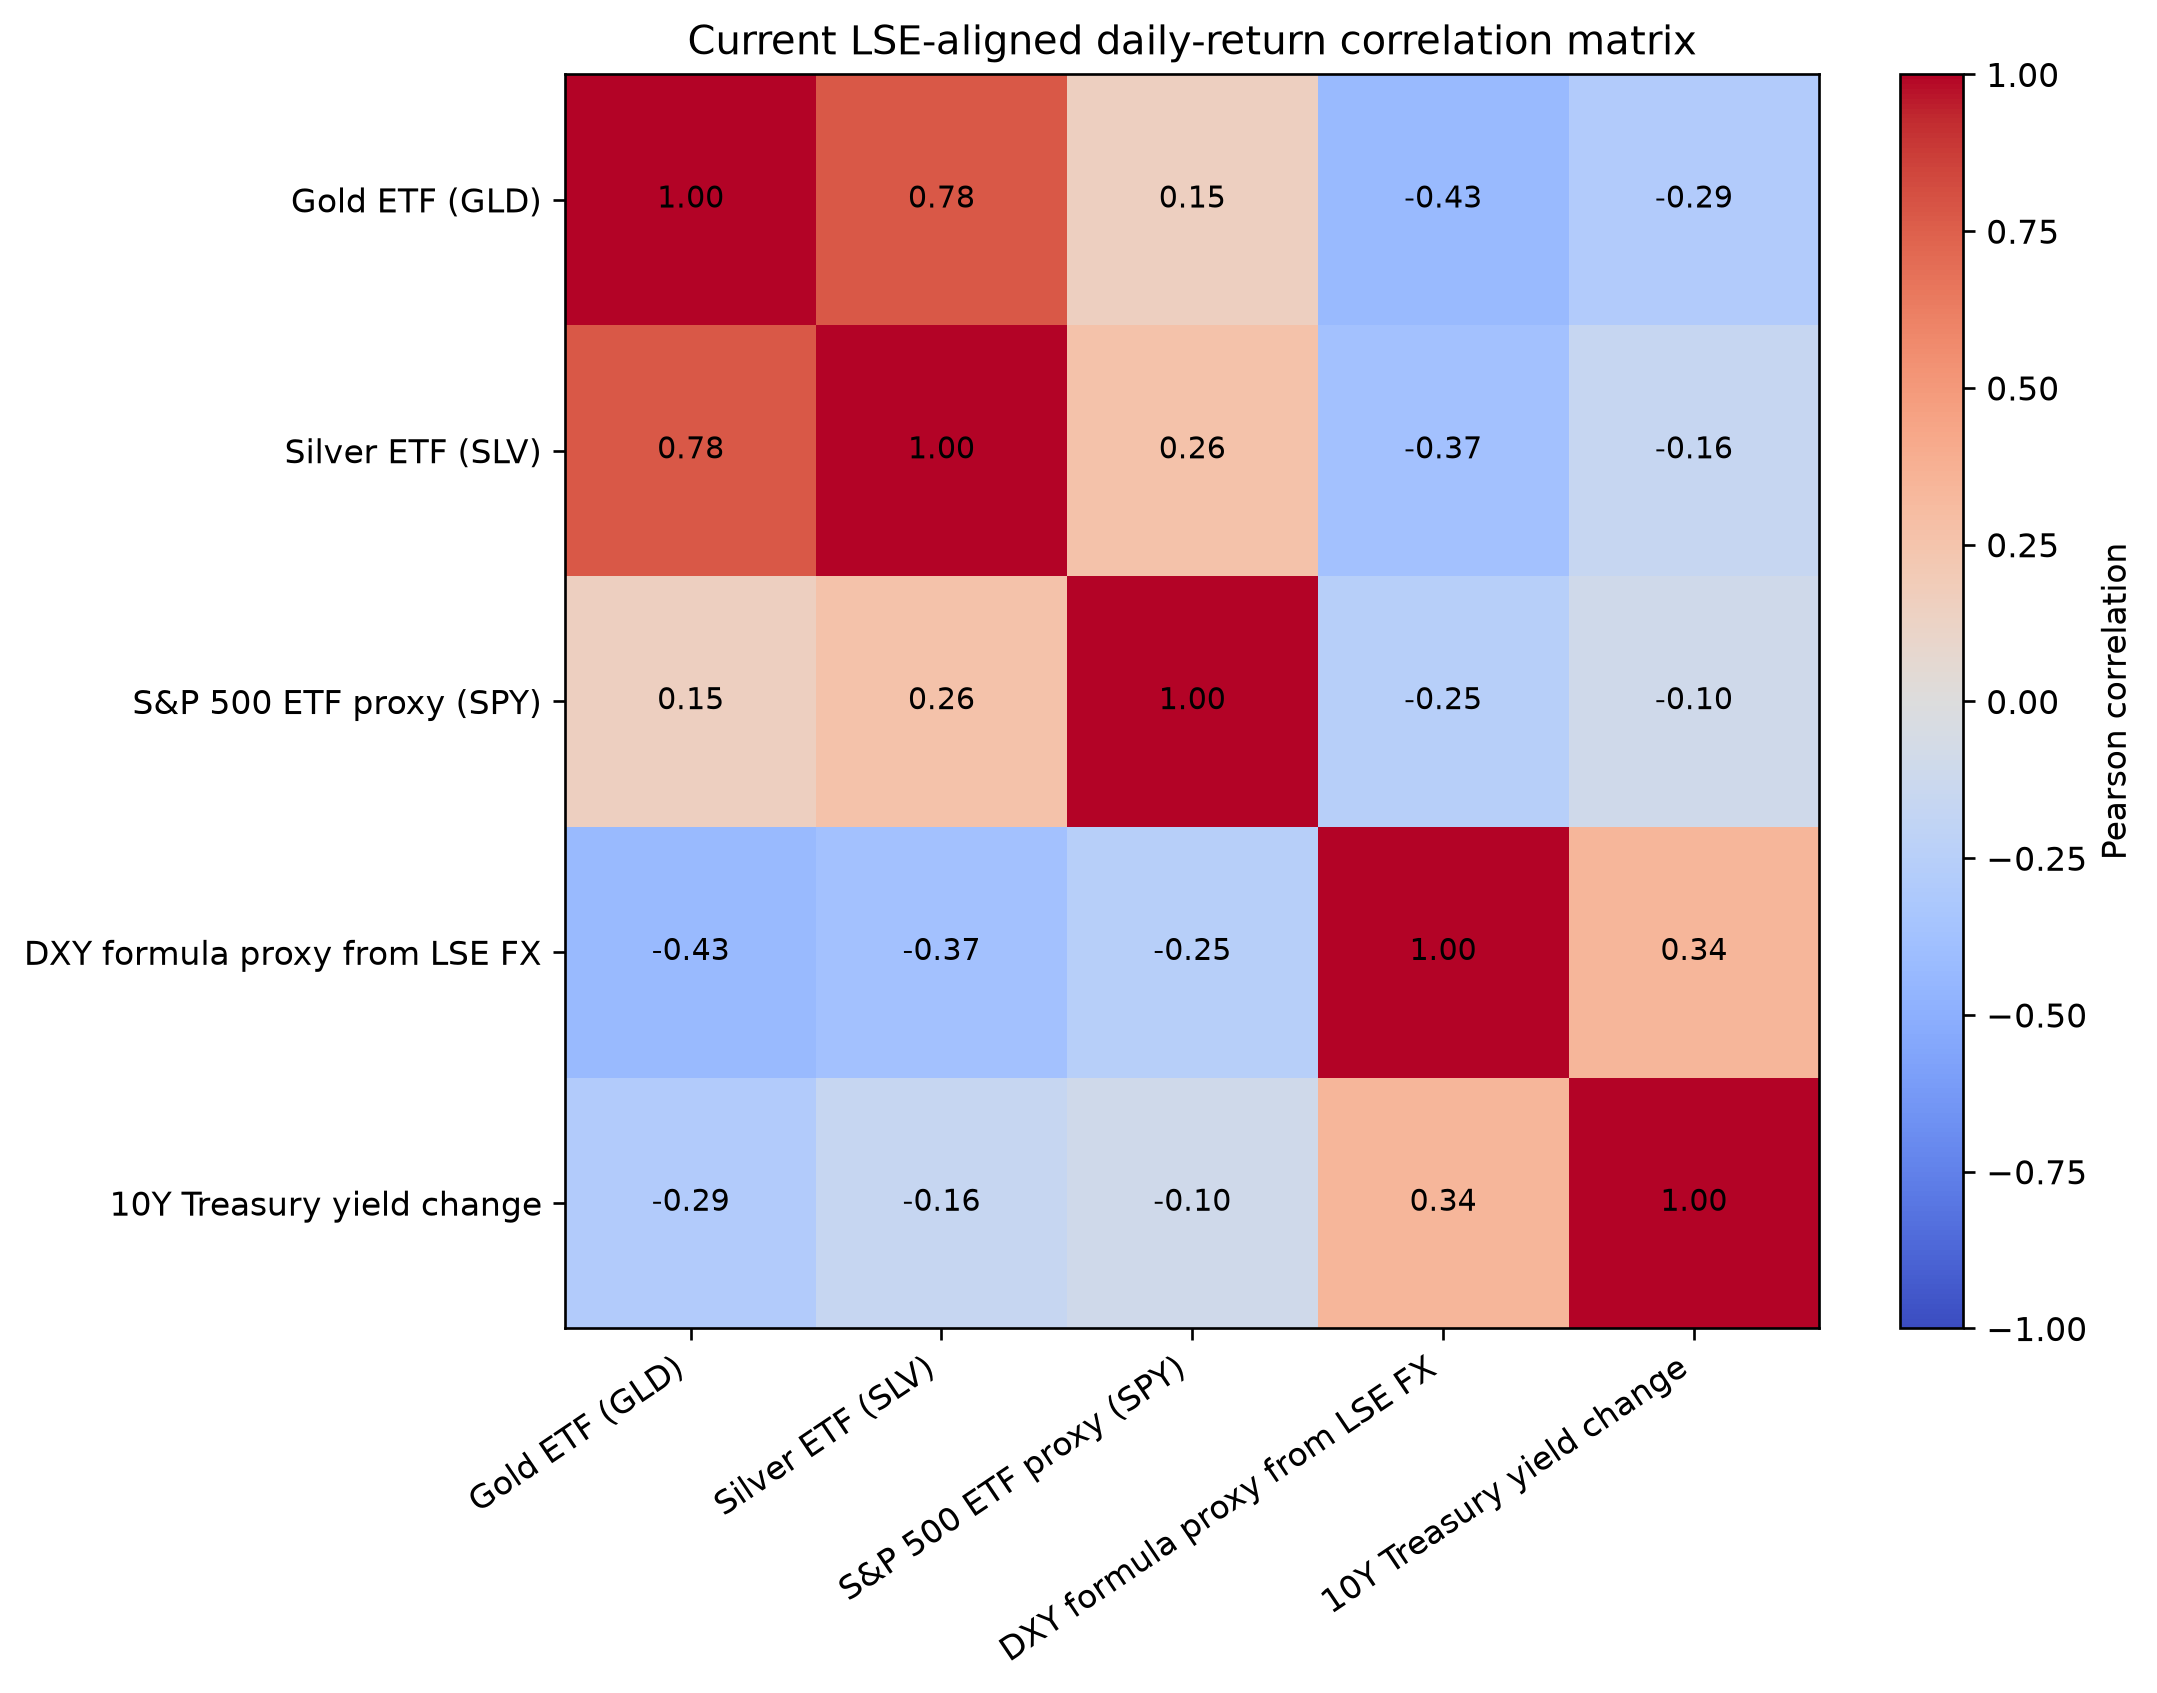
\includegraphics[width=0.82\textwidth]{../img/publication/208a6c6457382403_correlation_heatmap.png}
\caption{Static correlation matrix for the synchronized daily sample}
\label{fig:t7-correlation-heatmap}
\end{figure}

The current LSE matrix in Figure~\ref{fig:t7-correlation-heatmap} reveals
several patterns. GLD and SLV exhibit a strong positive correlation ($0.78$).
GLD is weakly correlated with SPY ($0.15$), while its correlations with the
DXY-formula proxy ($-0.43$) and the change in the 10-year Treasury yield
($-0.29$) are negative. SLV has a larger positive SPY correlation ($0.26$), a
negative dollar-proxy correlation ($-0.37$), and a weaker yield-change
correlation ($-0.16$). These are unconditional sample
associations, not universal hedge coefficients; the rolling evidence below
shows that both sign and magnitude vary through time.
\subsubsection{Linear regression framework}


Building on the correlation analysis discussed above, we next specify linear regression models that relate gold and silver returns to the macro-financial drivers identified in Chapter~\ref{ch:gold-regimes} and formalized econometrically in Chapter~\ref{ch:econometrics}.
While correlations are symmetric and purely descriptive, regression models impose a
direction of explanation and allow us to condition on multiple variables at once
\cite{Wooldridge2020}. Following the econometric framework introduced in the theoretical
section on ordinary least squares, we model gold and silver returns as linear functions of
the daily 10-year yield change and equity and dollar log returns:
\[
r^{gold}_t = \beta_0 + \beta_1 \Delta y_t + \beta_2 r^{equity}_t
+ \beta_3 r^{usd}_t + u_t,
\]
\[
r^{silver}_t = \gamma_0 + \gamma_1 \Delta y_t + \gamma_2 r^{equity}_t
+ \gamma_3 r^{usd}_t + v_t,
\]
where $u_t$ and $v_t$ denote error terms capturing all other factors that affect precious–
metal returns but are not explicitly included in the specification. These baseline models
allow us to quantify how gold and silver co–move with fixed–income markets, stock markets,
and the US dollar, holding the other drivers constant.

From a conceptual standpoint, the interpretation of the coefficients can follow two
complementary perspectives. A \emph{causal} interpretation would require strong identifying
assumptions on the error terms and on the absence of omitted variables, as emphasized in
the discussion of the zero conditional mean assumption and omitted variable bias in the
OLS framework. In this chapter, we primarily adopt a \emph{predictive} and descriptive
perspective: the coefficients are interpreted as measures of conditional co–movement and as
indicators of hedge and safe–haven properties, rather than as structural causal effects
(see also the distinction between causal and forecasting objectives in standard
econometrics and time–series texts, e.g.,~\cite{Wooldridge2020,Tsay2010}).

\section{Applied Cross-Asset Evidence}

Static correlations conceal economically important changes in sign and
magnitude. Figure~\ref{fig:t7-gold-rolling-correlations} regenerates the three
GLD rolling-correlation series from the current LSE panel. The dollar relation is
predominantly negative, whereas the equity and yield-change relations are more
state dependent. No rolling correlation alone identifies a causal channel.

\begin{figure}[htbp]
\centering
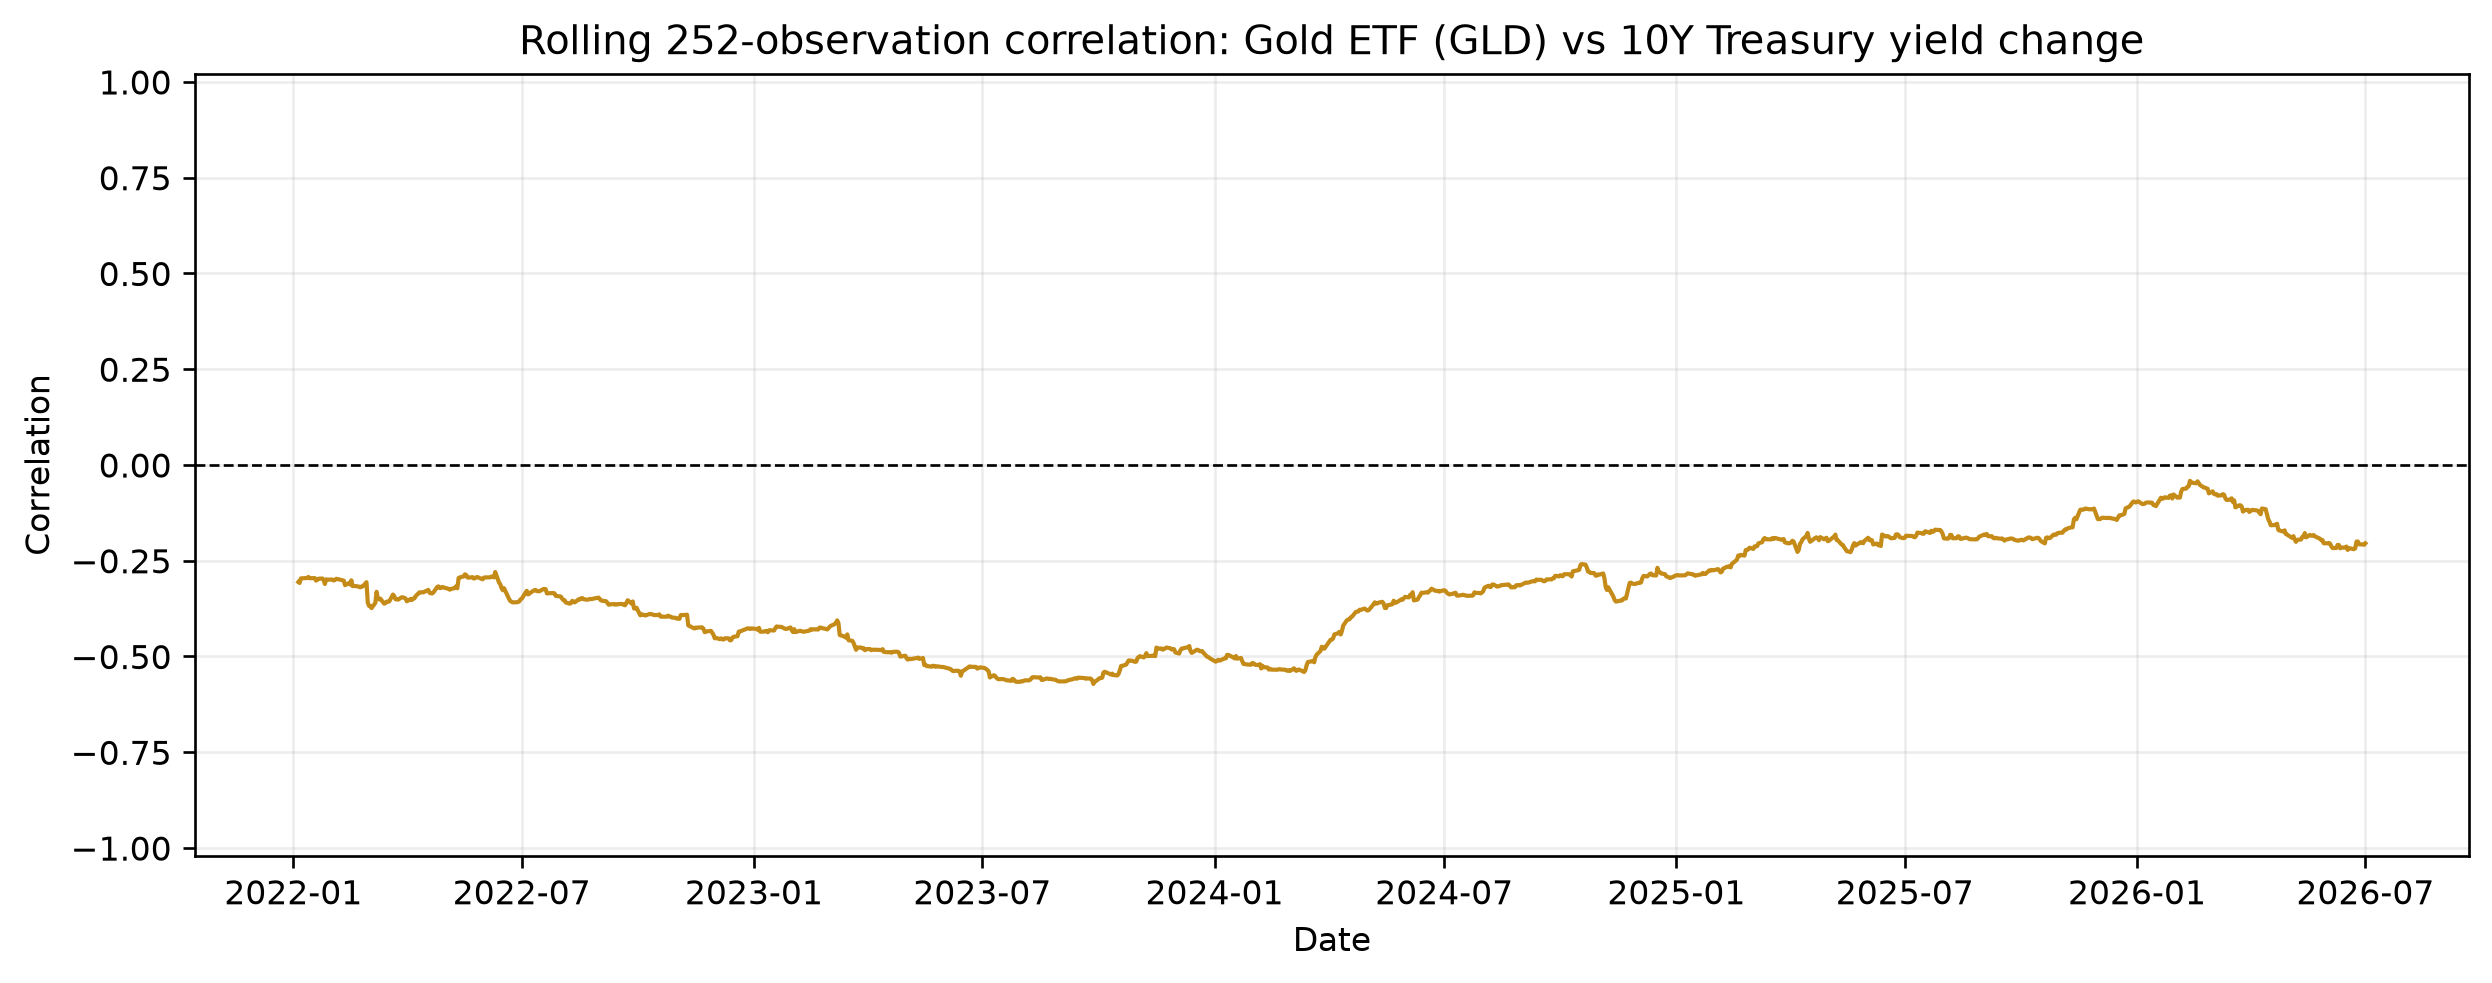
\includegraphics[width=0.88\textwidth]{../img/publication/15e8739a9649573e_rolling_corr_gold_ust10y.png}
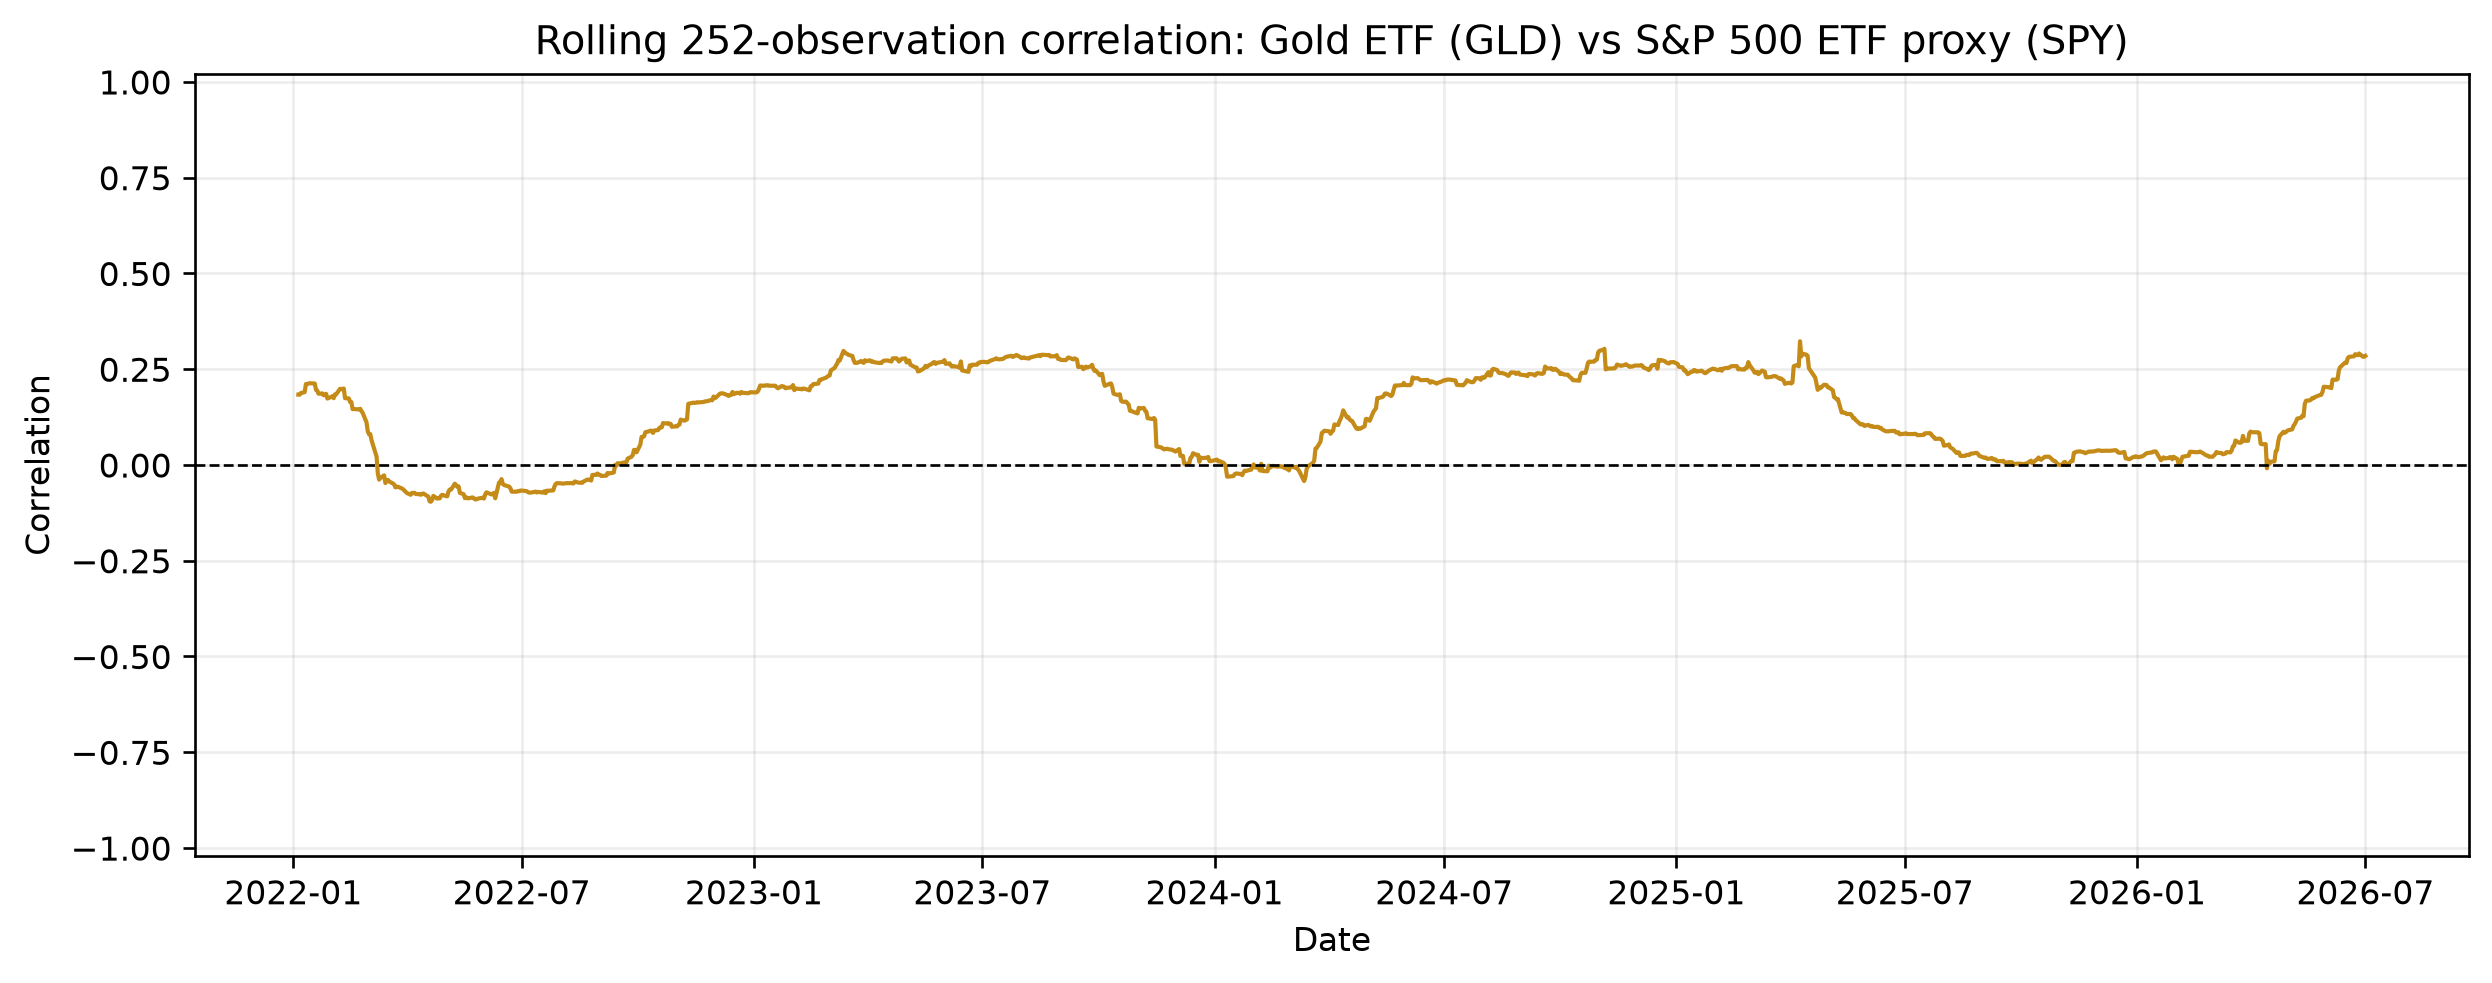
\includegraphics[width=0.88\textwidth]{../img/publication/cac8e0c90c783576_rolling_corr_gold_sp500.png}
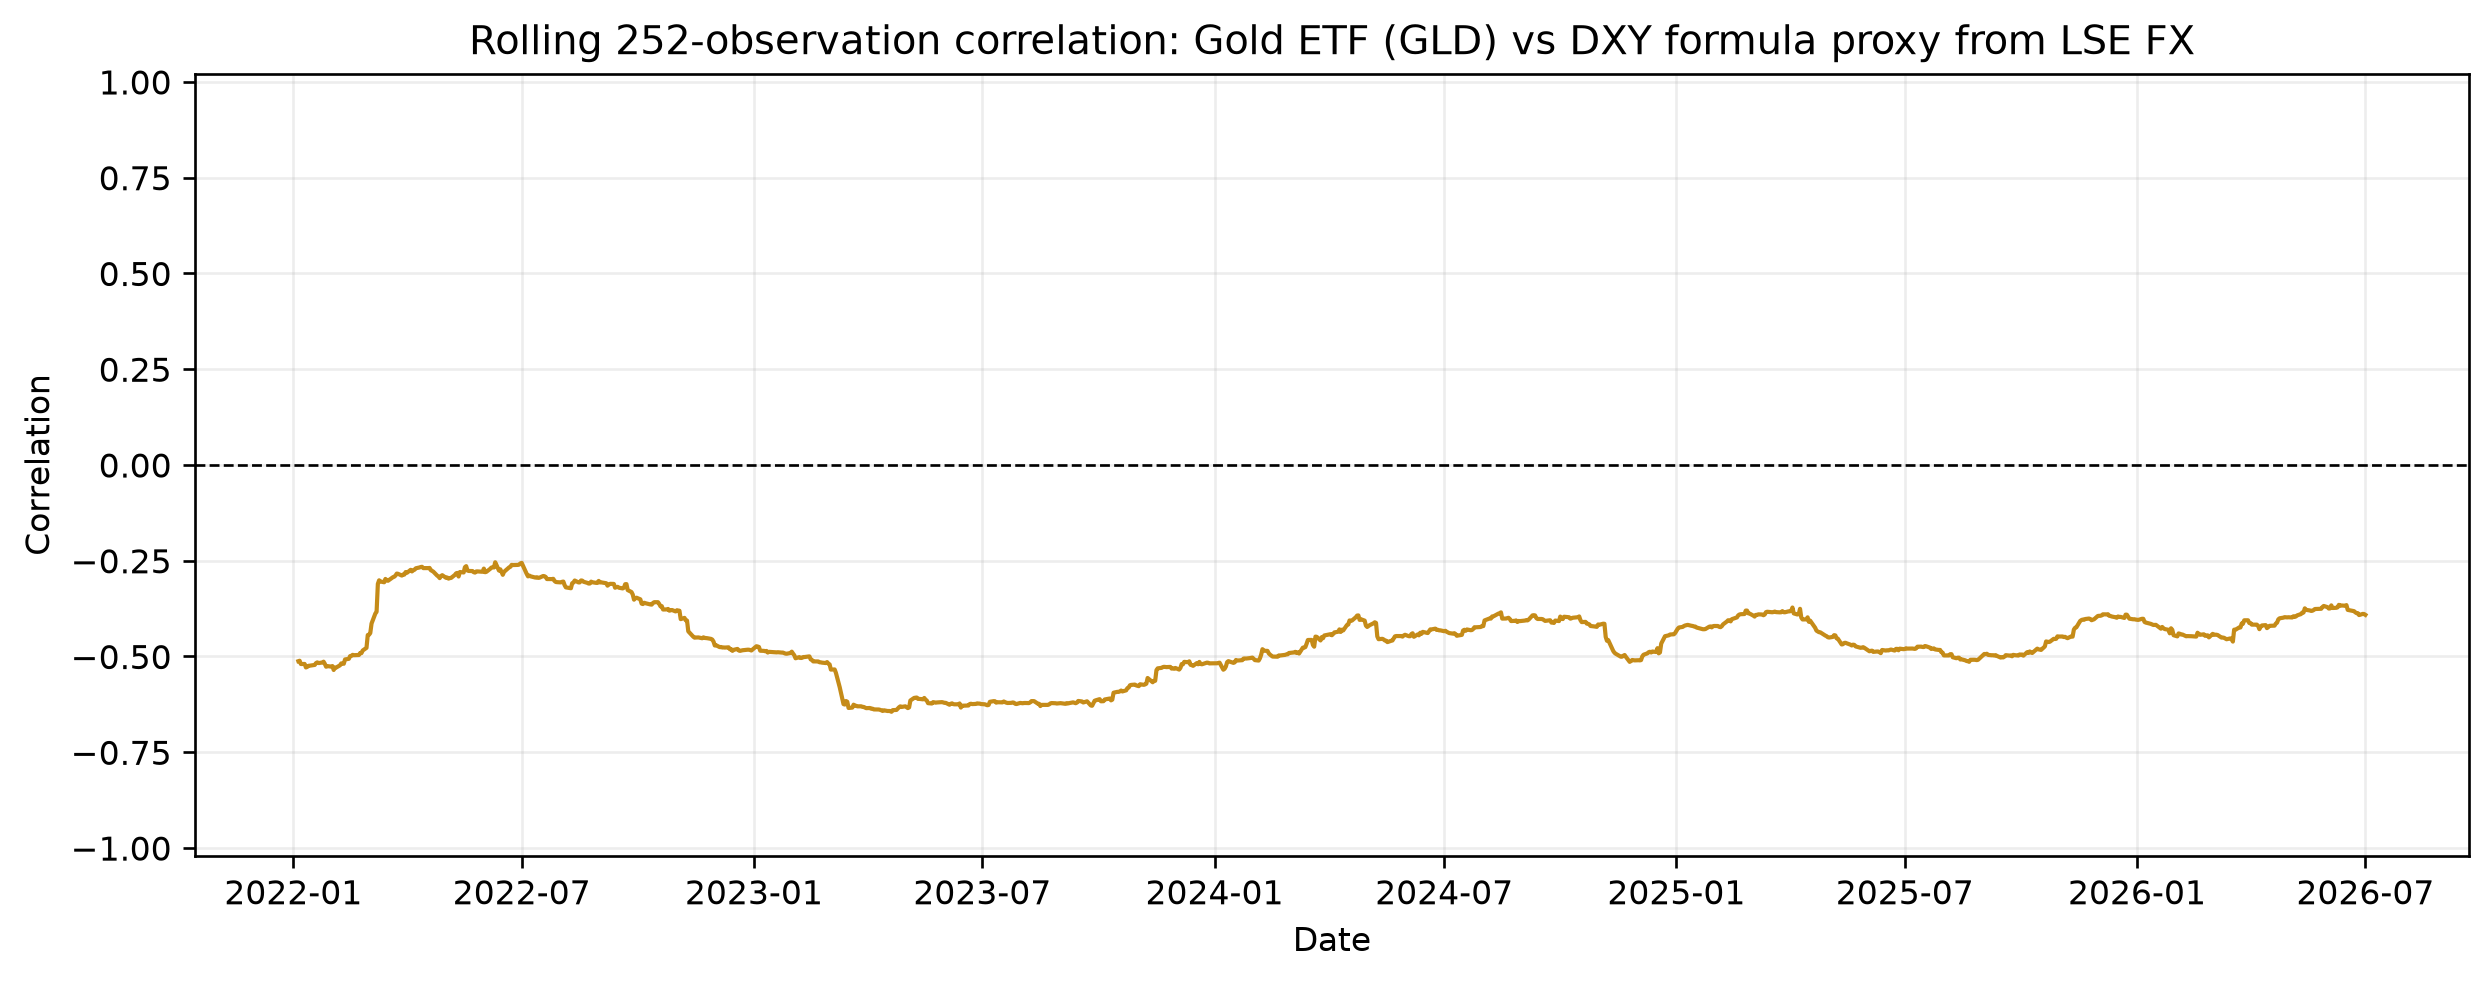
\includegraphics[width=0.88\textwidth]{../img/publication/f289761147385bd7_rolling_corr_gold_dxy.png}
\caption{Rolling 252-observation correlations of GLD returns with LSE
Treasury-yield changes, SPY returns and the transparent DXY-formula proxy}
\label{fig:t7-gold-rolling-correlations}
\end{figure}

The regression estimates in Table~\ref{tab:t7-gold-ols} quantify these
associations. Individually, gold loads negatively on yield changes and DXY;
the single-factor equity coefficient is small and positive. In the joint
specification, the DXY and yield-change coefficients remain statistically
different from zero, while the equity coefficient does not. The dollar factor
accounts for most of the reported explanatory power.

\begin{table}[htbp]
\centering
\caption{Gold-return regressions in the Team~7 sample}
\label{tab:t7-gold-ols}
\small
\begin{tabular}{lrrrr}
\toprule
 & Yield only & Equity only & Dollar only & Joint \\
\midrule
Yield change & $-0.0375^{***}$ & --- & --- & $-0.0292^{***}$ \\
             & $(0.0039)$      &     &     & $(0.0036)$       \\
S\&P 500 return & --- & $0.0506^{**}$ & --- & $0.0224$ \\
                &     & $(0.0250)$    &     & $(0.0250)$ \\
DXY return   & --- & --- & $-0.9810^{***}$ & $-0.9248^{***}$ \\
             &     &     & $(0.0450)$       & $(0.0466)$       \\
Constant     & $0.0003^{*}$ & $0.0003$ & $0.0003^{**}$ & $0.0003^{**}$ \\
             & $(0.0002)$   & $(0.0002)$& $(0.0001)$    & $(0.0001)$    \\
\midrule
$N$          & 4,694 & 4,694 & 4,694 & 4,694 \\
$R^2$        & 0.038 & 0.003 & 0.176 & 0.197 \\
Adjusted $R^2$ & 0.0376 & 0.0026 & 0.1760 & 0.1961 \\
\bottomrule
\end{tabular}
\begin{minipage}{0.92\textwidth}
\footnotesize\emph{Notes:} Heteroskedasticity-robust HC1 standard errors in
parentheses. $^{*}p<0.10$, $^{**}p<0.05$, $^{***}p<0.01$.
\end{minipage}
\end{table}

Silver provides a useful comparator rather than a substitute for gold. Its
rolling relations in Figure~\ref{fig:t7-silver-rolling-correlations} are more
equity-sensitive and remain time varying. In the joint regressions, silver's
equity loading is $0.2625$ (robust standard error $0.0424$), compared with
$0.0224$ ($0.0250$) for gold; the dollar loadings are $-1.6229$ ($0.0860$)
and $-0.9248$ ($0.0466$), respectively. The joint $R^2$ values are $0.205$
for silver and $0.197$ for gold.

\begin{table}[htbp]
\centering
\caption{Silver-return regressions in the Team~7 sample}
\label{tab:t7-silver-ols}
\small
\begin{tabular}{lrrrr}
\toprule
 & Yield only & Equity only & Dollar only & Joint \\
\midrule
Yield change & $-0.0206^{***}$ & --- & --- & $-0.0201^{***}$ \\
             & $(0.0067)$      &     &     & $(0.0062)$       \\
S\&P 500 return & --- & $0.3543^{***}$ & --- & $0.2625^{***}$ \\
                &     & $(0.0408)$     &     & $(0.0424)$       \\
DXY return   & --- & --- & $-1.7854^{***}$ & $-1.6229^{***}$ \\
             &     &     & $(0.0789)$        & $(0.0860)$        \\
Constant     & $0.0001$ & $0.0000$ & $0.0002$ & $0.0001$ \\
             & $(0.0002)$& $(0.0003)$& $(0.0002)$& $(0.0002)$ \\
\midrule
$N$          & 4,694 & 4,694 & 4,694 & 4,694 \\
$R^2$        & 0.004 & 0.049 & 0.182 & 0.205 \\
Adjusted $R^2$ & 0.0030 & 0.0485 & 0.1810 & 0.2050 \\
\bottomrule
\end{tabular}
\begin{minipage}{0.92\textwidth}
\footnotesize\emph{Notes:} Heteroskedasticity-robust HC1 standard errors in
parentheses. $^{*}p<0.10$, $^{**}p<0.05$, $^{***}p<0.01$.
\end{minipage}
\end{table}

\begin{figure}[htbp]
\centering
\begin{minipage}{0.49\textwidth}
\centering
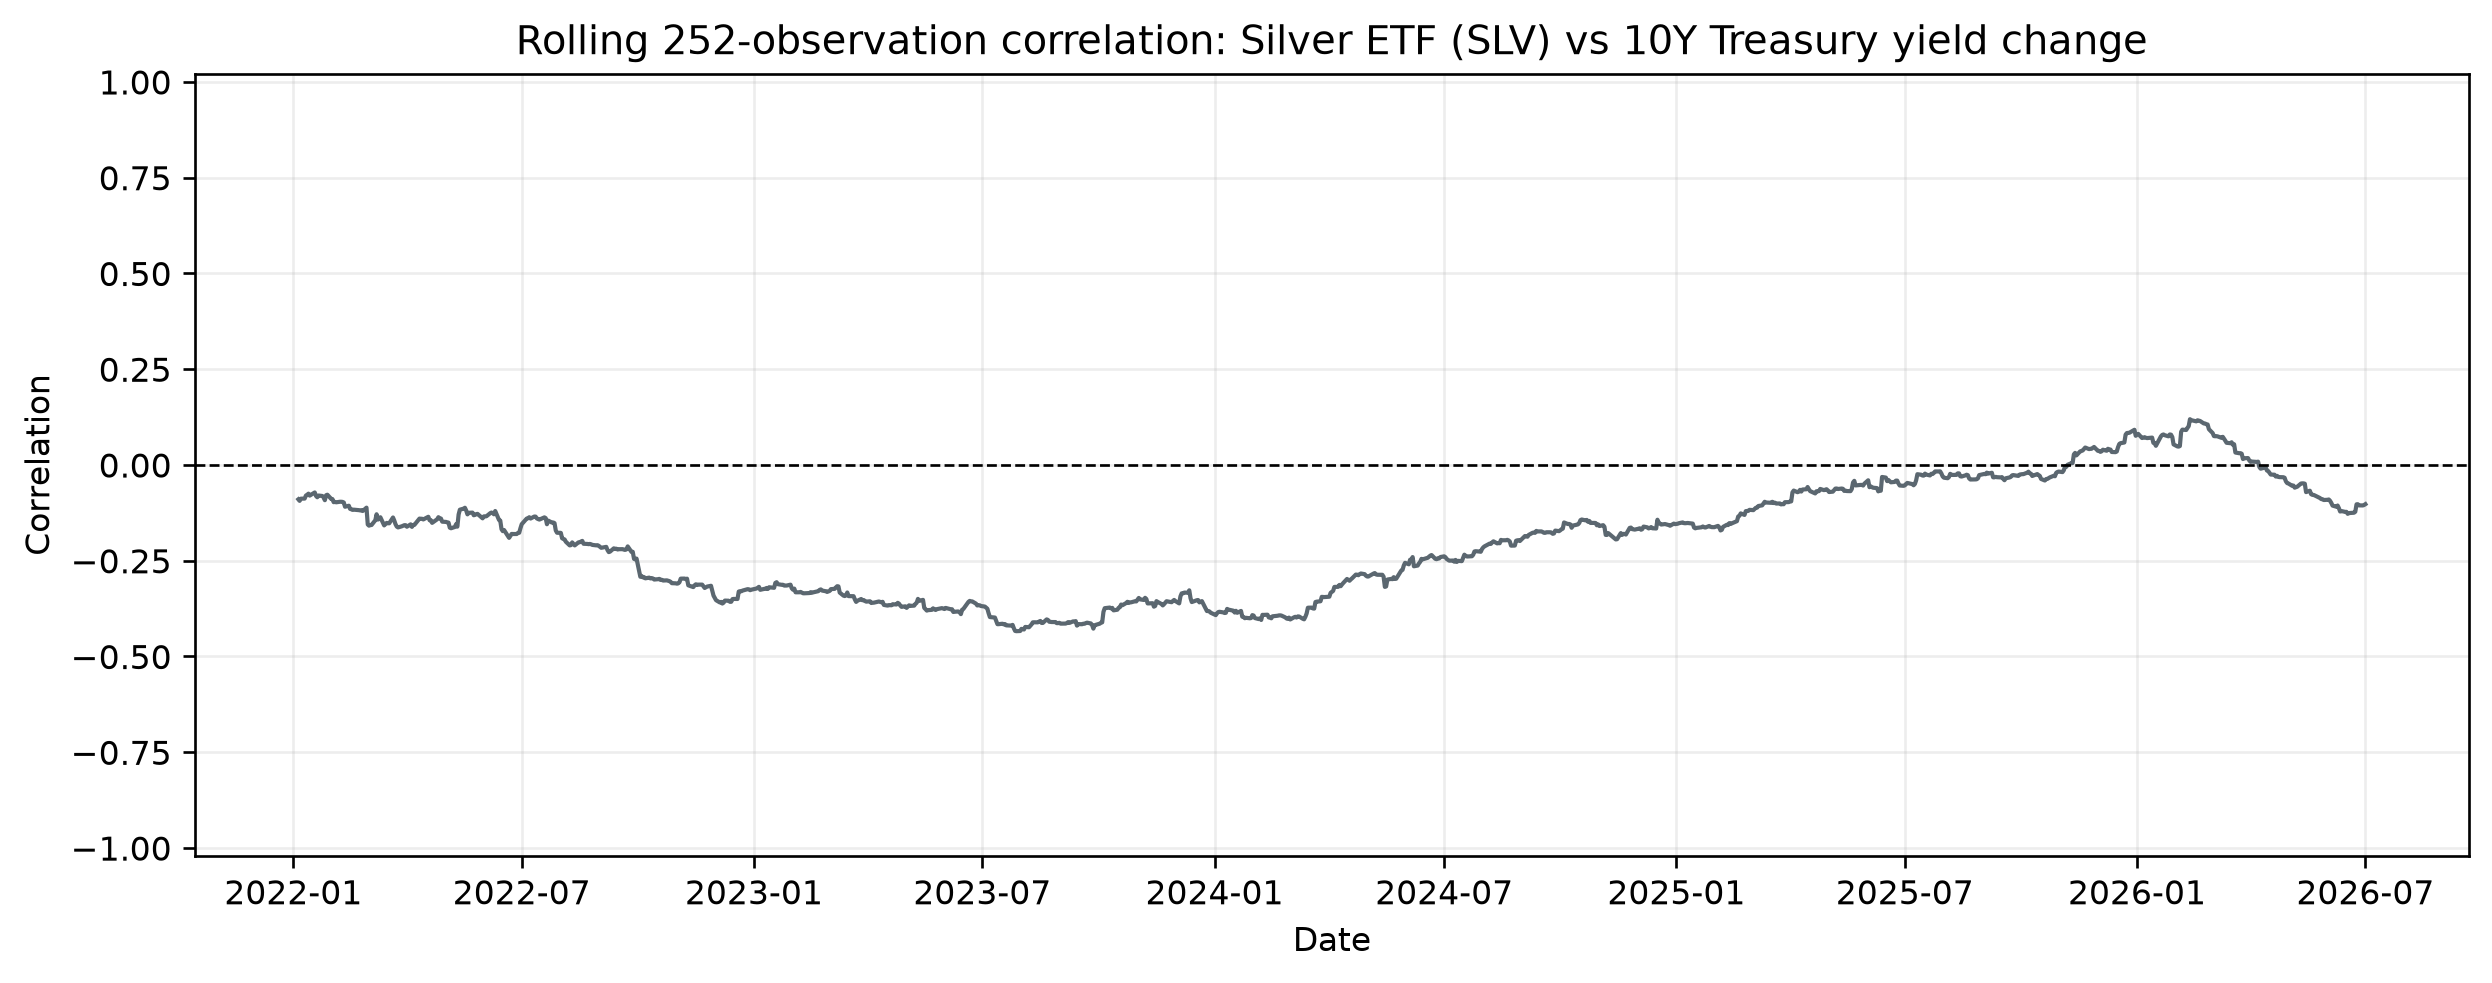
\includegraphics[width=\linewidth]{../img/publication/908c62e76c1ec216_rolling_corr_silver_ust10y.png}
\end{minipage}\hfill
\begin{minipage}{0.49\textwidth}
\centering
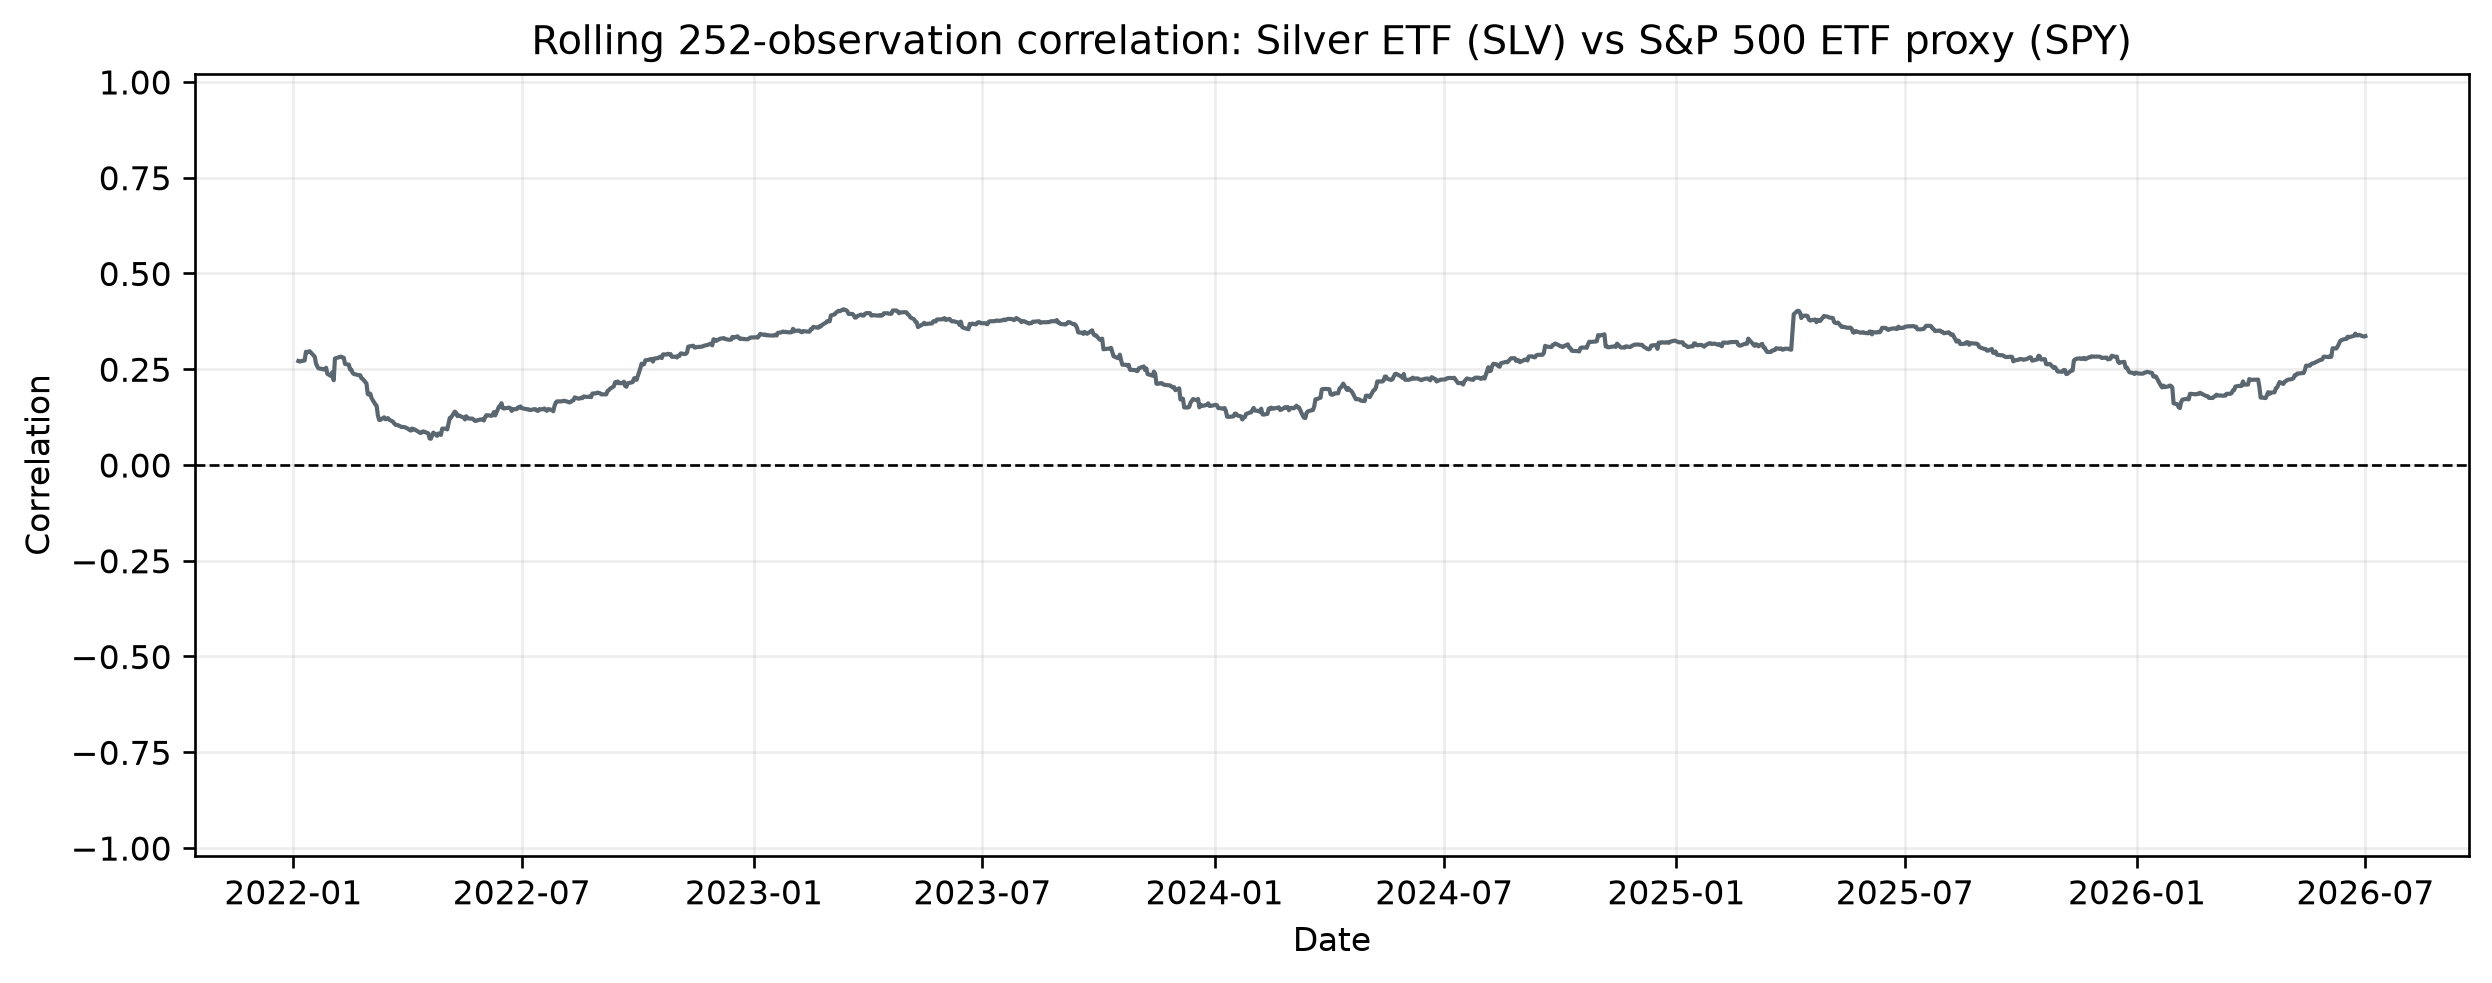
\includegraphics[width=\linewidth]{../img/publication/749384e5a43b524a_rolling_corr_silver_sp500.png}
\end{minipage}

\begin{minipage}{0.55\textwidth}
\centering
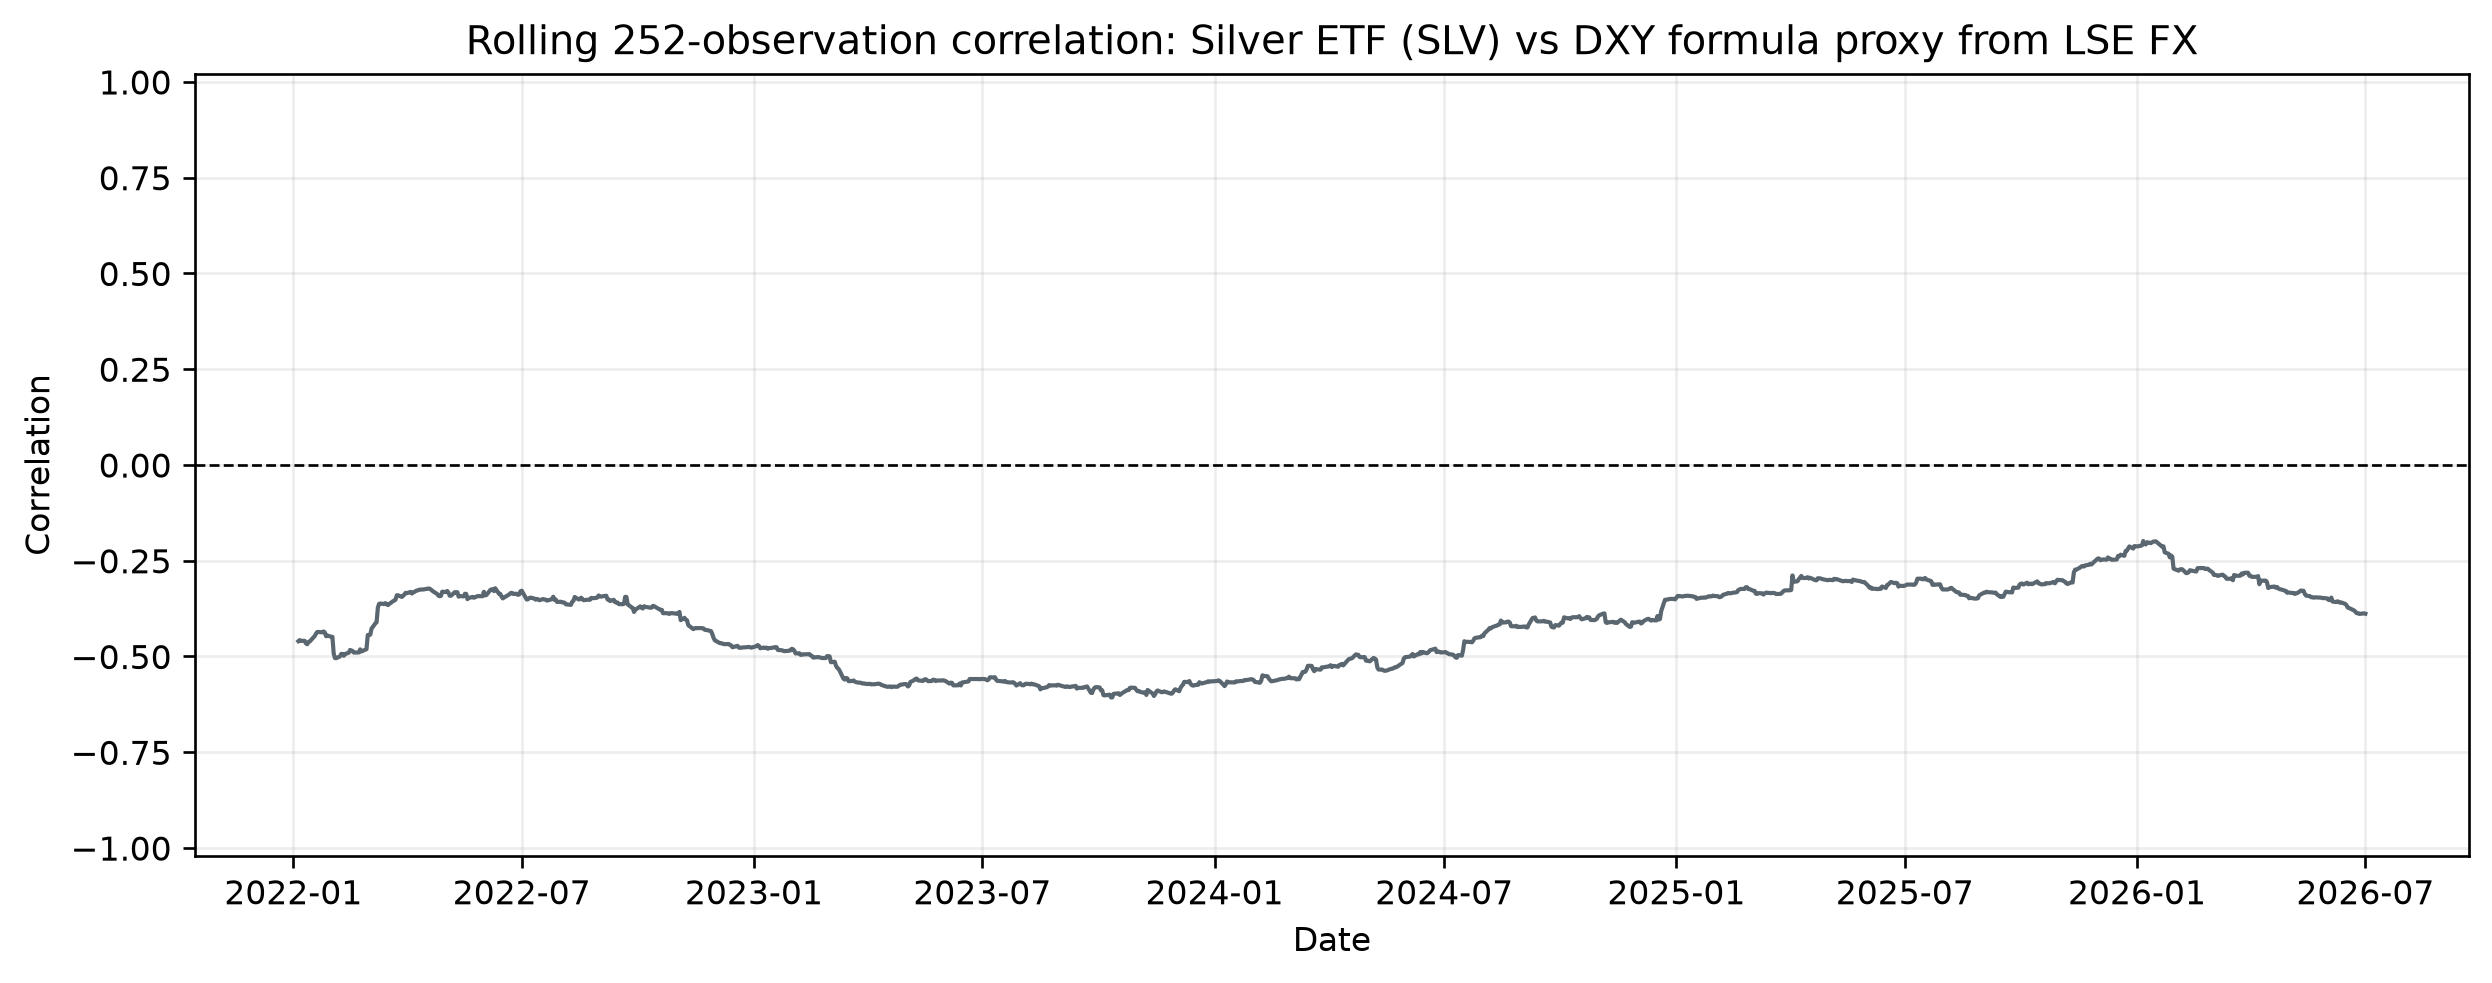
\includegraphics[width=\linewidth]{../img/publication/446a86ada886cf6f_rolling_corr_silver_dxy.png}
\end{minipage}
\caption{Rolling 252-observation correlations of SLV returns with LSE
Treasury-yield changes, SPY returns and the transparent DXY-formula proxy}
\label{fig:t7-silver-rolling-correlations}
\end{figure}

The combined evidence supports three limited conclusions. Gold and silver are
strongly related but silver is materially more volatile; gold's unconditional
equity relationship is weak; and the negative dollar relationship is much
more stable than the bond-yield or equity relations. The evidence motivates
state-dependent volatility modeling, but it does not establish a universal
safe-haven law.

\section{Log Prices, Returns and Stationarity}

The distinction between log-price levels and log returns governs the model
choice. Log prices are highly persistent and empirically close to a unit-root
process, whereas daily returns are much closer to weak stationarity. An AR(1)
fit to price levels consequently produces coefficients near one and very high
in-sample explanatory power: approximately $0.9993$ for gold with
$R^2\approx0.999$, and $0.9978$ for silver with $R^2\approx0.996$. These values
primarily record persistence and must not be read as useful economic
forecastability.

For returns, the same benchmark changes sharply. The estimated AR(1)
coefficient is approximately $-0.0024$ for gold and $0.0063$ for silver, with
published robust standard errors near $0.0202$ and $0.0227$ and essentially zero
$R^2$. At the daily frequency the conditional mean is therefore weak even
though the price level is persistent.

\begin{table}[htbp]
\centering
\caption{AR(1) contrast between log-price levels and daily returns}
\label{tab:t7-ar1-level-return}
\small
\begin{tabular}{llrrrr}
\toprule
Asset & Dependent series & $\hat\phi_1$ & Robust s.e. & $t$-statistic & $R^2$ \\
\midrule
Gold   & Log price & 0.9993  & 0.0006 & 1653.18 & 0.9987 \\
Silver & Log price & 0.9978  & 0.0012 &  802.26 & 0.9956 \\
Gold   & Return    &-0.0024  & 0.0202 &   -0.12 & 0.0000 \\
Silver & Return    & 0.0063  & 0.0227 &    0.28 & 0.0000 \\
\bottomrule
\end{tabular}
\begin{minipage}{0.90\textwidth}
\footnotesize\emph{Notes:} Cells reproduce the published Team~7 article.
The corrected companion code reports Newey--West HAC standard errors and
$t$-statistics of 0.000587/1703.3 (gold) and 0.001228/812.7 (silver) for
log prices, and 0.01942/$-0.124$ (gold) and 0.02480/0.255 (silver) for
returns. Coefficients and $R^2$ agree at the shown precision, and no
significance conclusion changes. High fit in levels reflects near-unit-root
persistence, not reliable return predictability.
\end{minipage}
\end{table}

\section{AR, ARMA and ARIMA Diagnostics}

Higher-order autoregressions do not overturn the AR(1) result. AIC and BIC
select low-dimensional specifications and the joint lag tests provide little
evidence that lagged daily returns explain current returns. ARMA searches also
remain parsimonious and are not stable enough across criteria to reveal a
substantive conditional-mean law.

\begin{table}[htbp]
\centering
\caption{Higher-order autoregressive diagnostics for daily returns}
\label{tab:t7-arp-diagnostics}
\small
\begin{tabular}{lrrrrr}
\toprule
Asset & AIC lag & BIC lag & $R^2$ & Joint $F$ & $p$-value \\
\midrule
Gold   & 1 & 1 & 0.000006 & 0.0144 & 0.9046 \\
Silver & 1 & 1 & 0.000040 & 0.0779 & 0.7801 \\
\bottomrule
\end{tabular}
\end{table}

ARIMA is not rejected because prices are non-stationary: differencing is
precisely how the model addresses that feature. On log prices, the legacy
selection produces ARIMA$(2,1,0)$ by AIC and ARIMA$(0,1,1)$ by BIC for gold;
for silver both criteria select ARIMA$(1,1,0)$. Once differenced, these models
are close to the simple ARMA descriptions of returns and add little predictive
structure at the horizon considered.

\begin{table}[htbp]
\centering
\caption{Information-criterion selections for ARMA returns and ARIMA log prices}
\label{tab:t7-arma-arima-selection}
\small
\begin{tabular}{lllrr}
\toprule
Asset & Series and criterion & Selected order & AIC & BIC \\
\midrule
Gold   & Return, AIC      & ARMA$(2,0)$  & -28,909.4140 & --- \\
Gold   & Return, BIC      & ARMA$(0,1)$  & --- & -28,889.9939 \\
Silver & Return, AIC/BIC  & ARMA$(1,0)$  & -23,448.9424 & -23,429.5802 \\
Gold   & Log price, AIC   & ARIMA$(2,1,0)$ & -28,909.4140 & --- \\
Gold   & Log price, BIC   & ARIMA$(0,1,1)$ & --- & -28,889.9939 \\
Silver & Log price, AIC/BIC & ARIMA$(1,1,0)$ & -23,448.9424 & -23,429.5802 \\
\bottomrule
\end{tabular}
\begin{minipage}{0.94\textwidth}
\footnotesize\emph{Notes:} The equality of several ARMA and ARIMA criteria is
expected because first-differenced log prices are the return series. Dashes
mark the criterion not used for the stated selection.
\end{minipage}
\end{table}

\section{Heavy Tails, Clustering and Persistence}

The return distribution shifts attention from the conditional mean to the
second moment and the tails. In the published 2006--2024 table layer, daily standard deviation
is approximately $1.1\%$ for gold and $2.0\%$ for silver. Estimated skewness is
about $-0.33$ and $-0.85$, while excess kurtosis is approximately $6.25$ and
$7.79$. Gaussian innovations therefore understate the frequency and asymmetry
of large moves, especially for silver.

\begin{table}[htbp]
\centering
\caption{Distributional moments of daily precious-metal returns}
\label{tab:t7-return-moments}
\small
\begin{tabular}{lrrrrr}
\toprule
Asset & Mean & Std. dev. & Skewness & Excess kurtosis & Kurtosis \\
\midrule
Gold   & 0.00028 & 0.01112 & -0.33 & 6.25 & 9.25 \\
Silver & 0.00014 & 0.01990 & -0.85 & 7.79 & 10.79 \\
\bottomrule
\end{tabular}
\end{table}
The table preserves the source-PDF moments; saved CSV excess kurtosis is
6.23770 (gold) and 7.78276 (silver). The cause of this smaller discrepancy
is unverified; it is distinct from the AR(1) SE/$t$ divergence and does
not establish an error in the ARMA/ARIMA tables.

Figures~\ref{fig:t7-return-histograms} and
\ref{fig:t7-return-qqplots}, regenerated on current LSE GLD/SLV returns, make
the departure from Gaussianity visible. The
center is sharper than the fitted normal density and both tails contain more
mass; the Q--Q deviations are especially pronounced for silver.

\begin{figure}[htbp]
\centering
\begin{minipage}{0.49\textwidth}
\centering
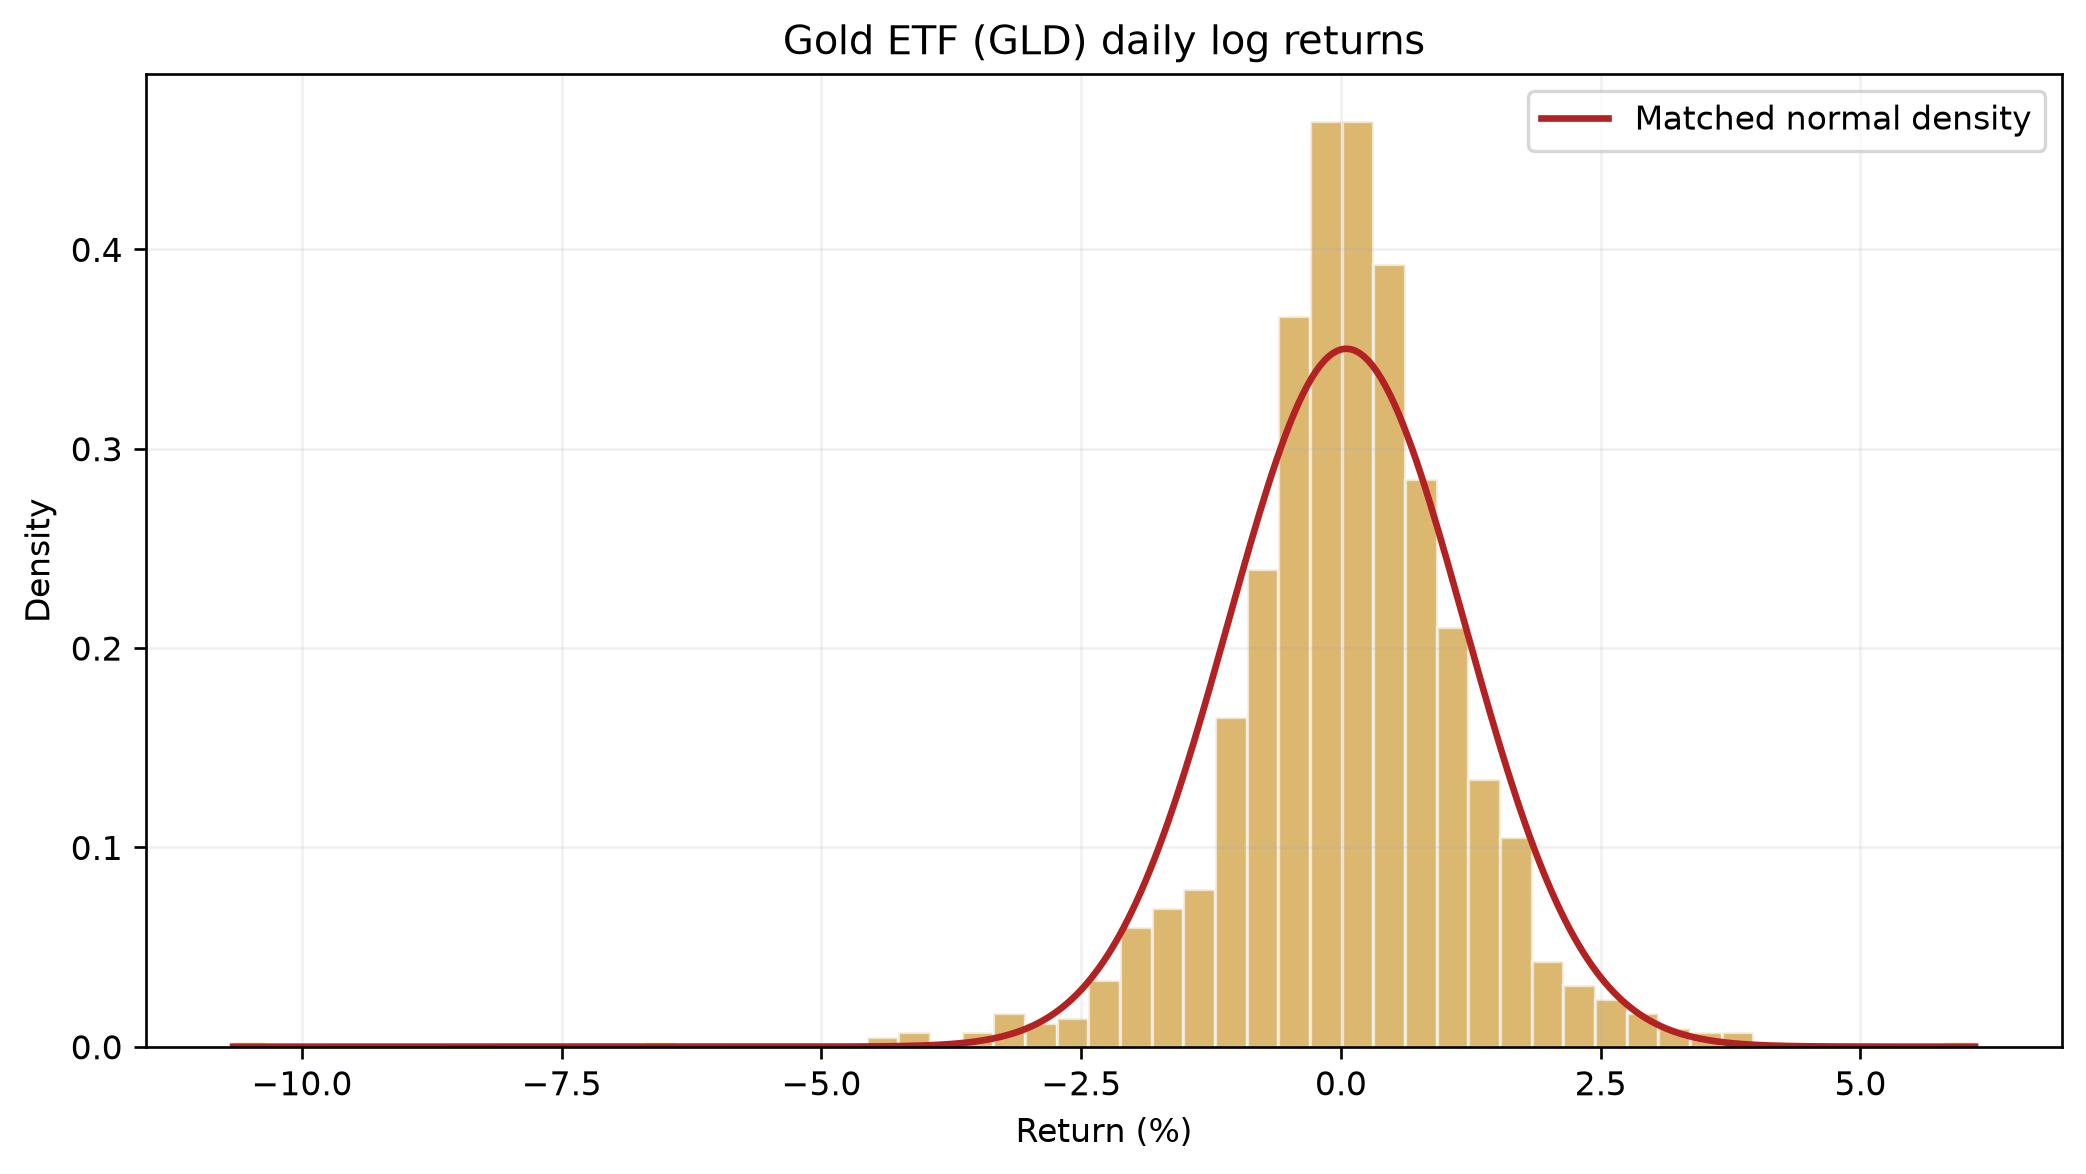
\includegraphics[width=\linewidth]{../img/publication/cade4f2733f97d8b_hist_normal_gold.png}
\end{minipage}\hfill
\begin{minipage}{0.49\textwidth}
\centering
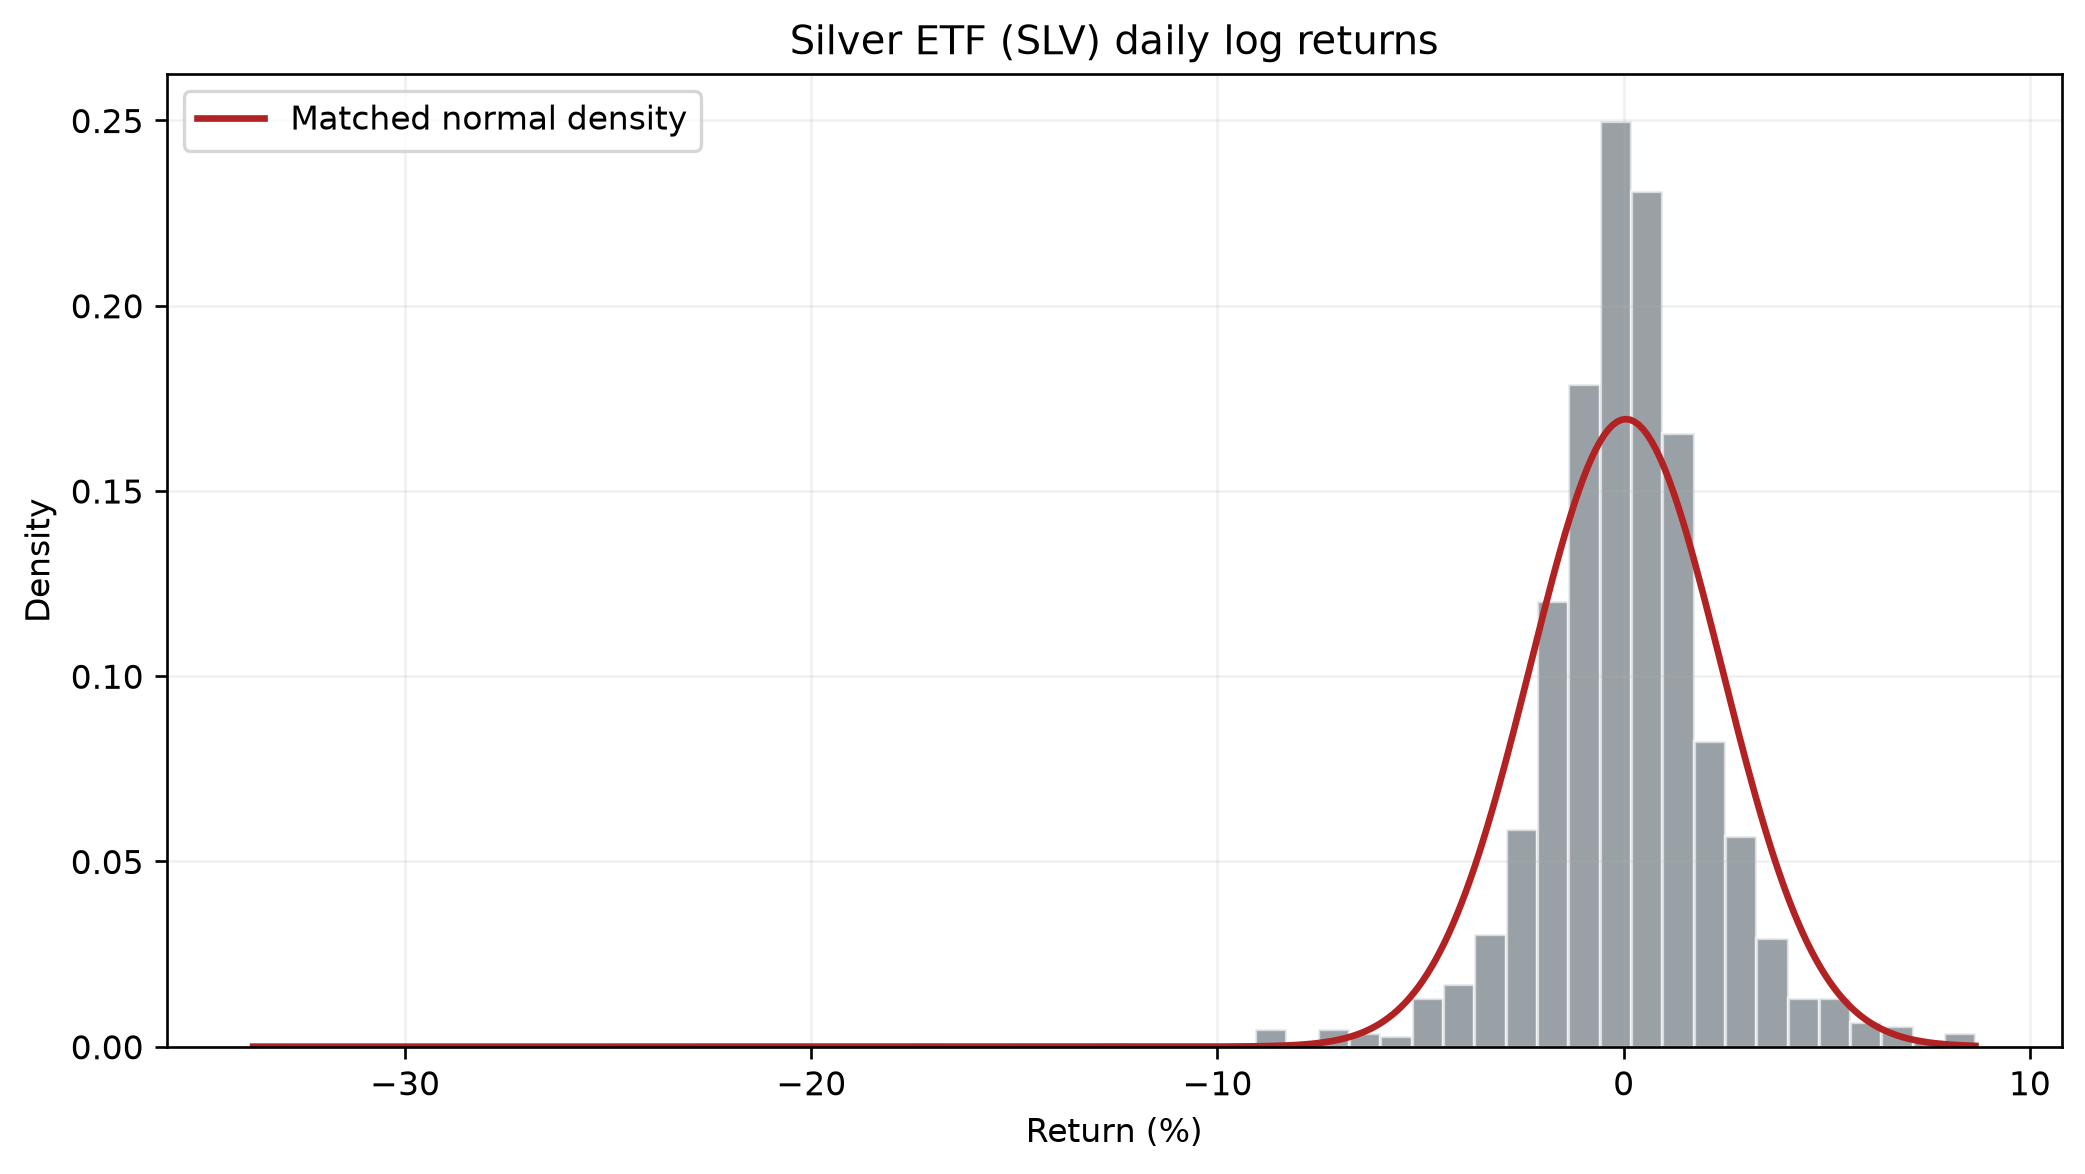
\includegraphics[width=\linewidth]{../img/publication/33a47b013cdc5552_hist_normal_silver.png}
\end{minipage}
\caption{Current LSE GLD and SLV return histograms with matched normal benchmarks}
\label{fig:t7-return-histograms}
\end{figure}

\begin{figure}[htbp]
\centering
\begin{minipage}{0.49\textwidth}
\centering
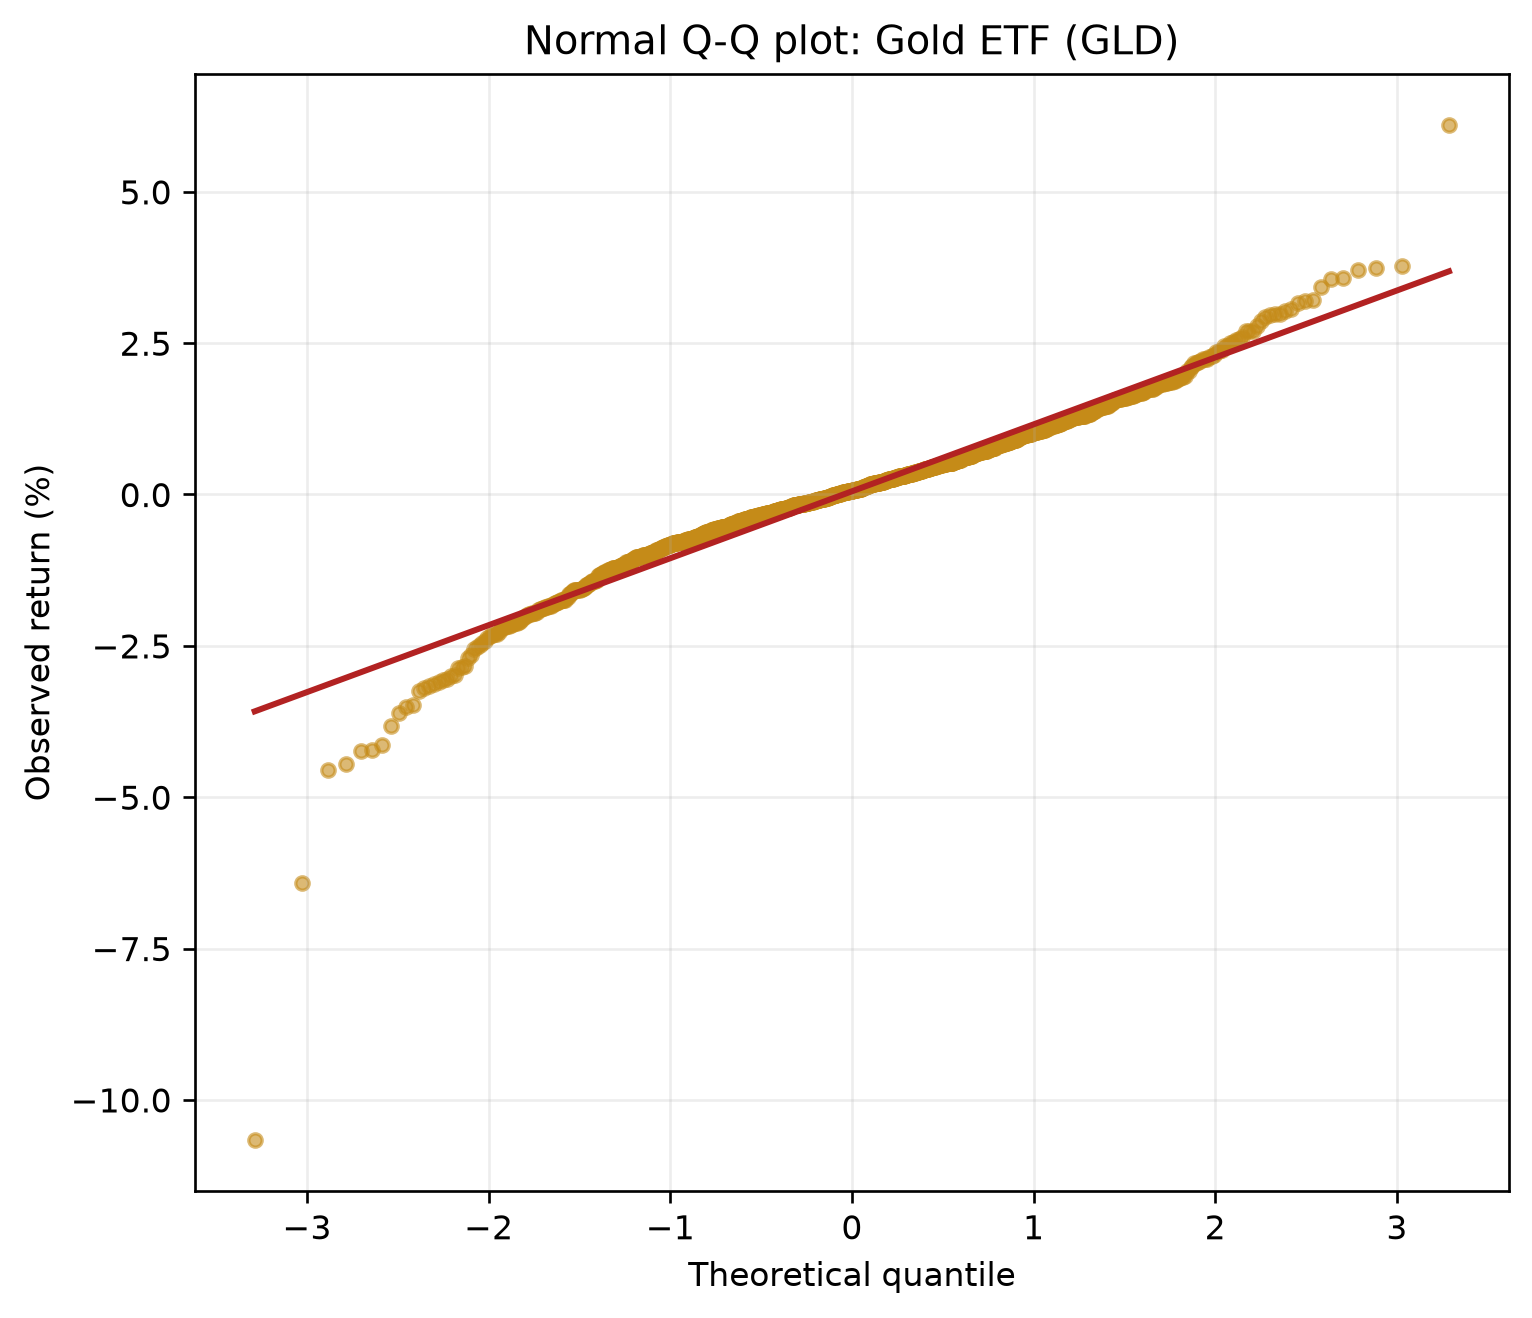
\includegraphics[width=\linewidth]{../img/publication/b634a7a755db7d7f_qqplot_normal_gold.png}
\end{minipage}\hfill
\begin{minipage}{0.49\textwidth}
\centering
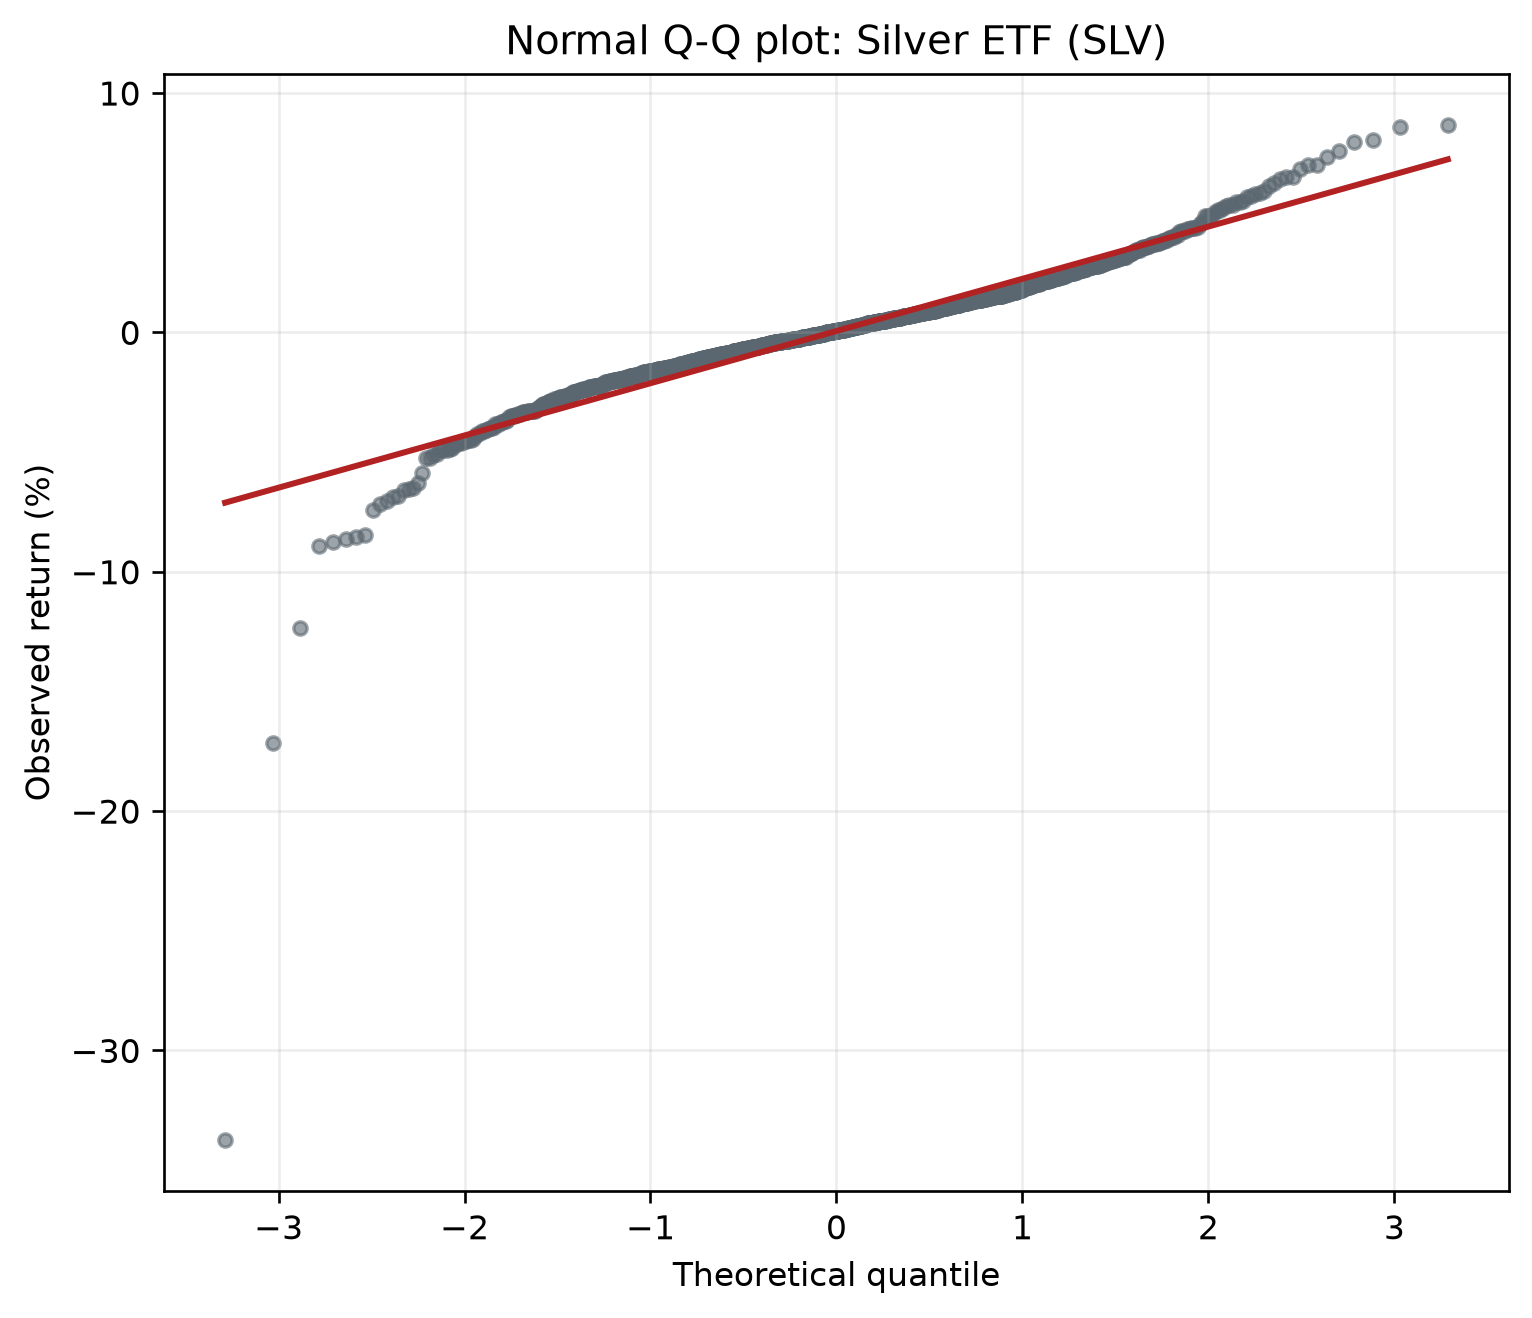
\includegraphics[width=\linewidth]{../img/publication/5a4373ae994c4282_qqplot_normal_silver.png}
\end{minipage}
\caption{Current LSE normal Q--Q diagnostics for GLD and SLV returns}
\label{fig:t7-return-qqplots}
\end{figure}

Absolute and squared returns show positive serial dependence even when raw
return autocorrelation is weak. Large changes tend to be followed by large
changes of either sign, and shocks decay slowly. This volatility clustering is
the empirical feature that a constant-variance mean model misses most clearly.

\begin{figure}[htbp]
\centering
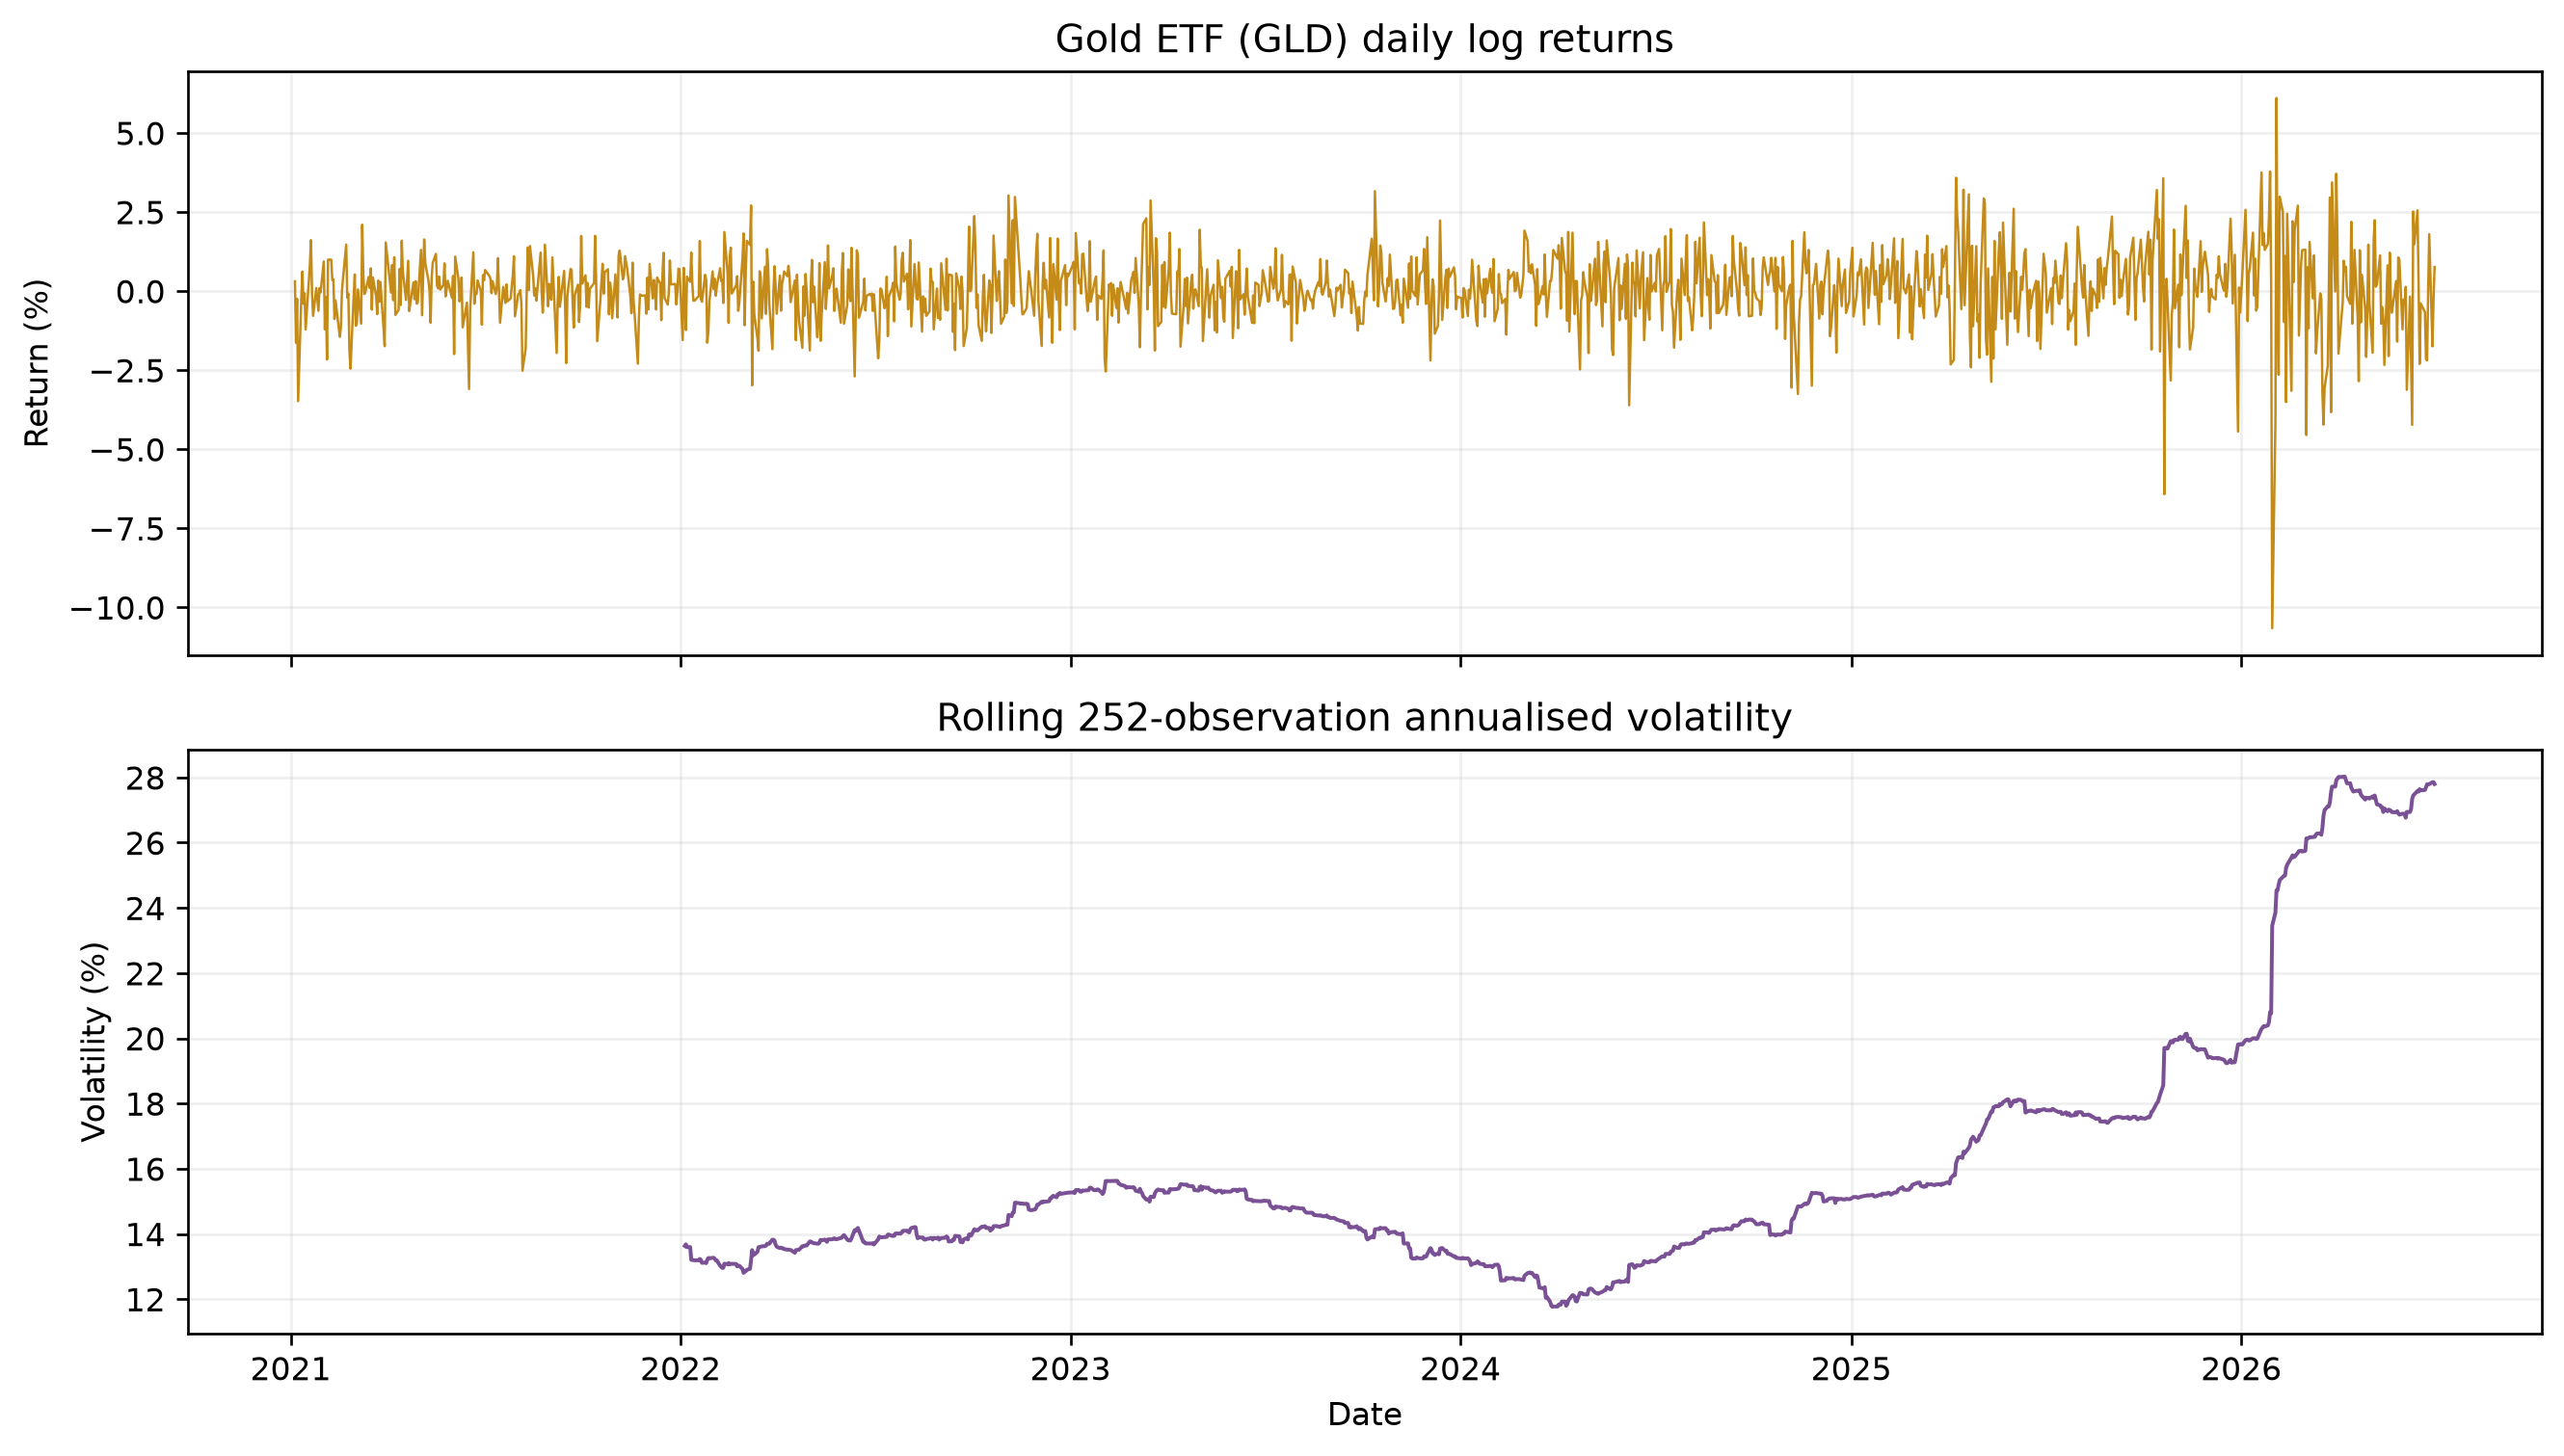
\includegraphics[width=0.88\textwidth]{../img/publication/e670a201ce86a5ec_returns_rollingvol_gold.png}
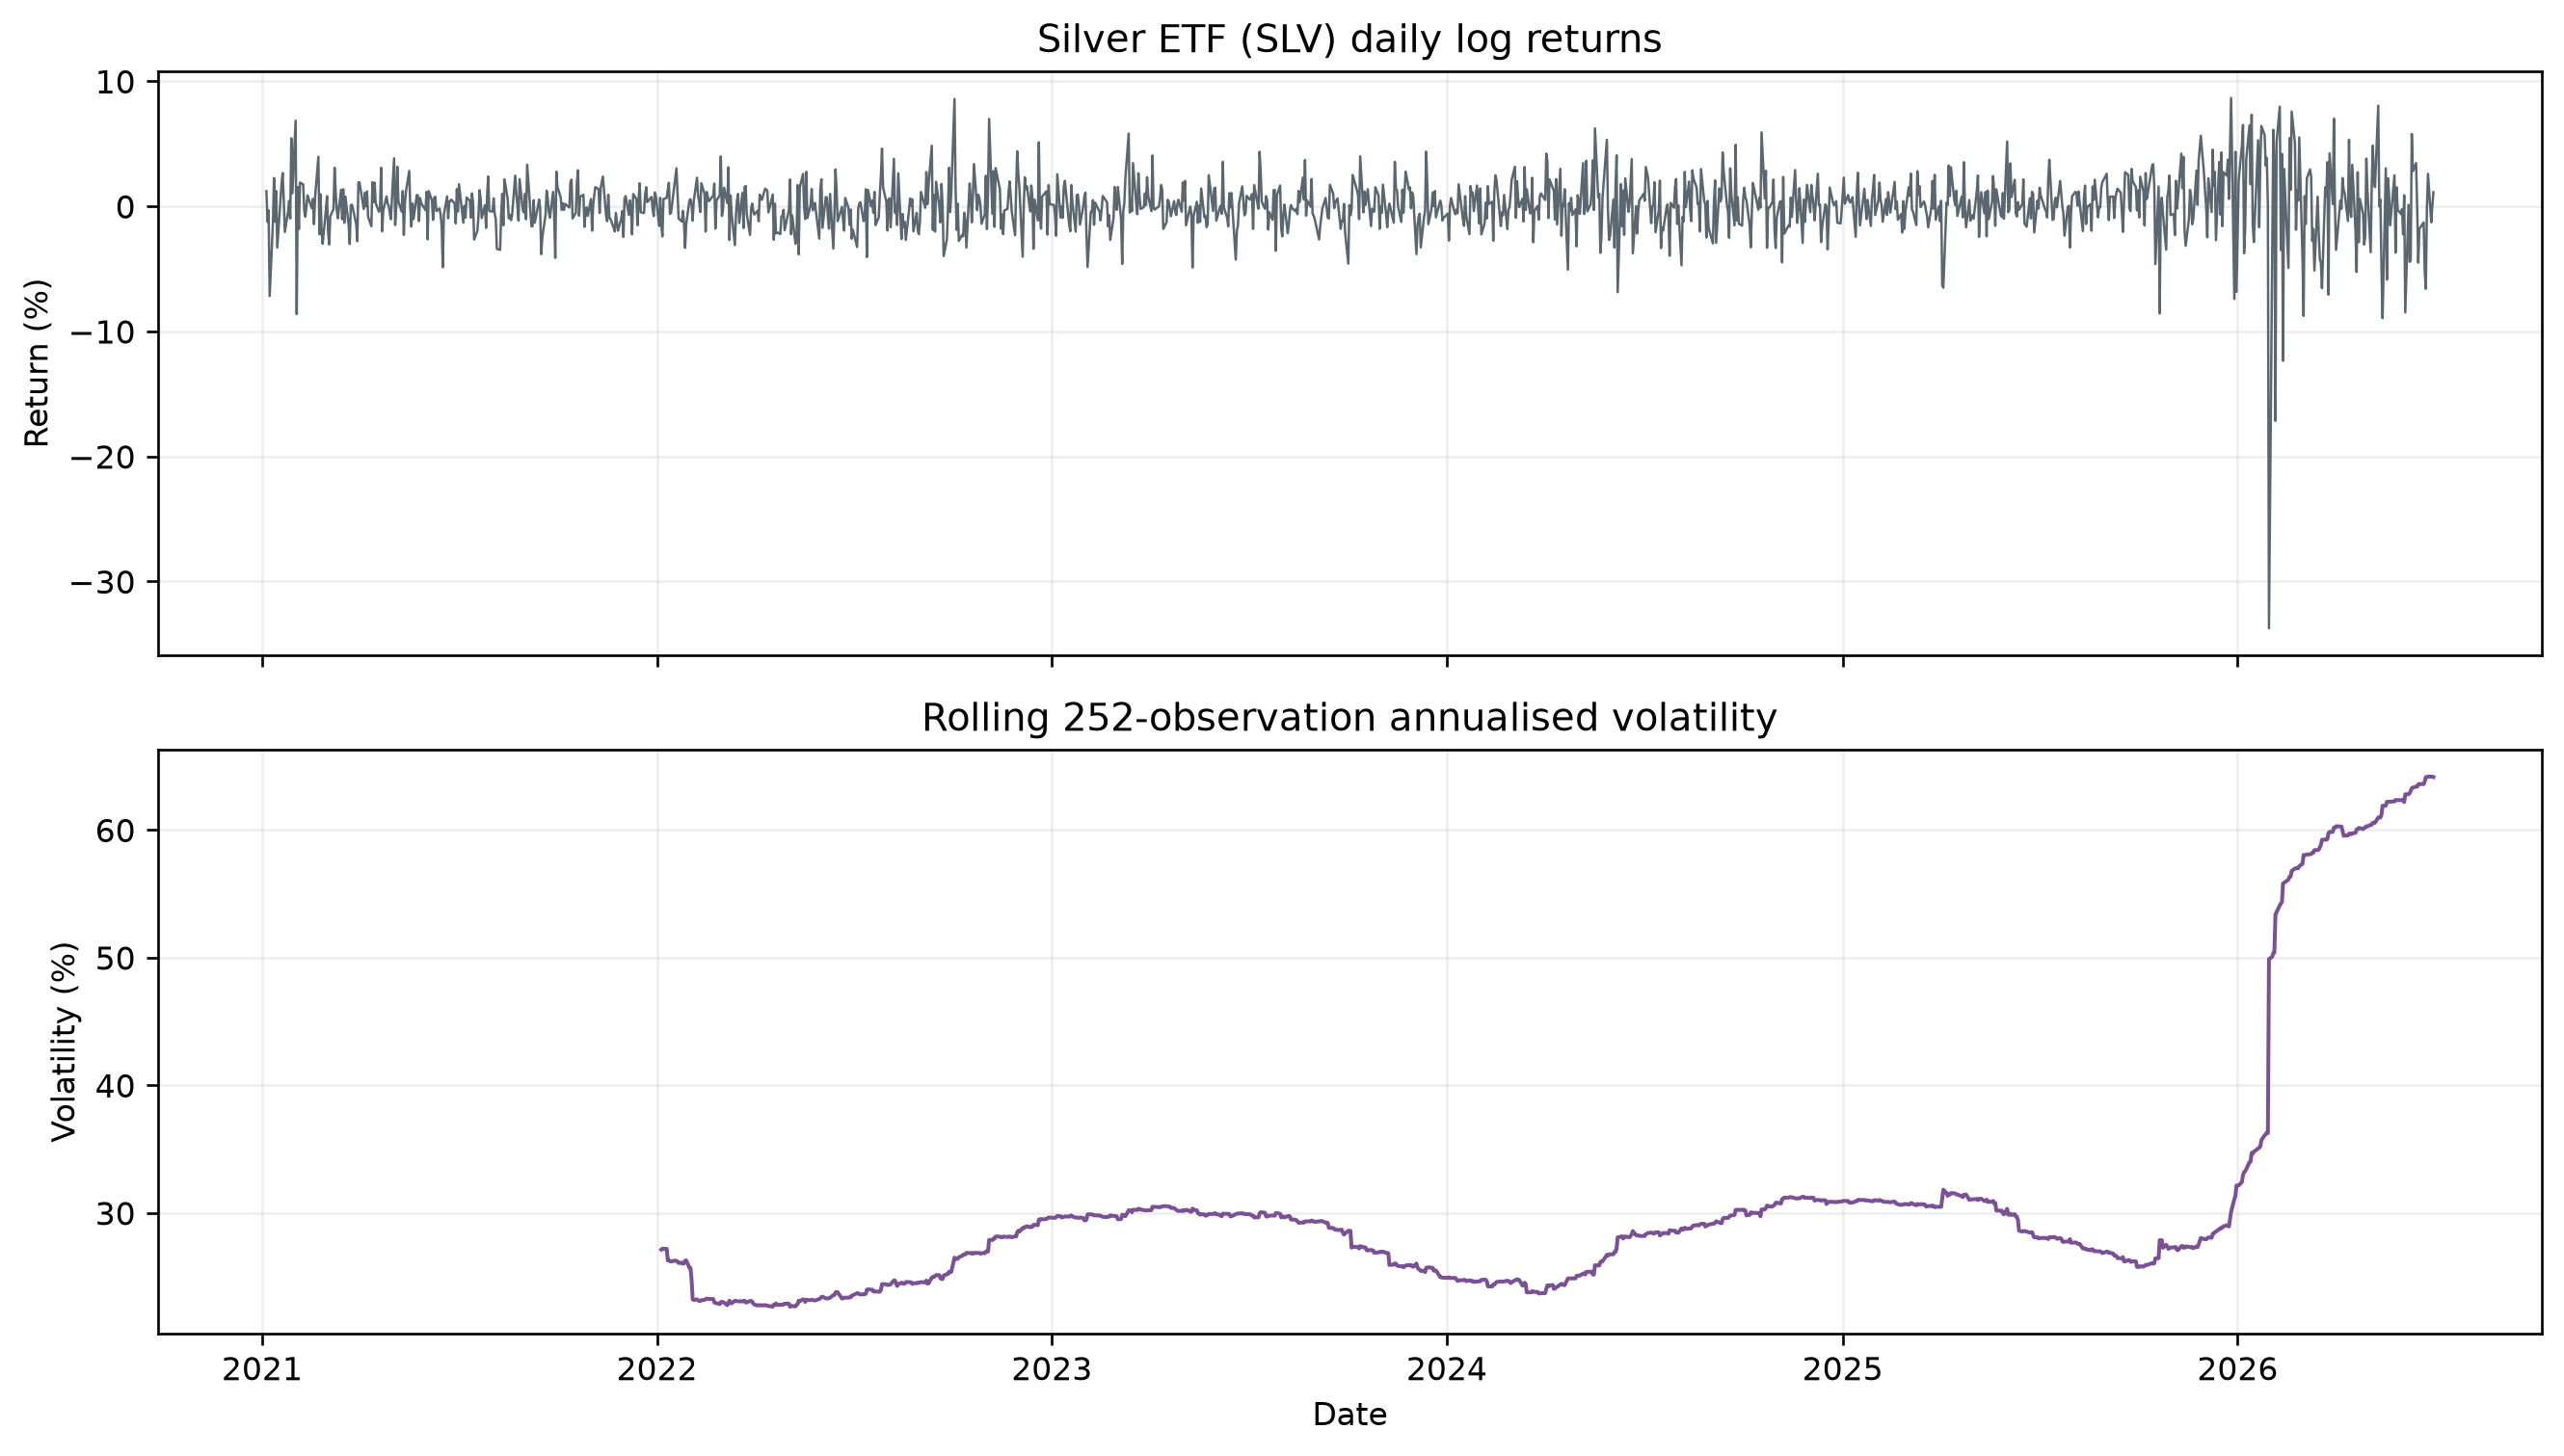
\includegraphics[width=0.88\textwidth]{../img/publication/a27b1fd9ae7d7a38_returns_rollingvol_silver.png}
\caption{Current LSE daily returns and rolling 252-observation annualized volatility for GLD and SLV}
\label{fig:t7-rolling-volatility}
\end{figure}

The ACF panels in Figure~\ref{fig:t7-acf-grid} separate the mean and variance
signals. Raw-return autocorrelations remain close to zero, whereas absolute
and squared returns retain positive dependence over many lags. The compact
persistence statistics in Table~\ref{tab:t7-persistence} reach the same
conclusion.

\begin{figure}[htbp]
\centering
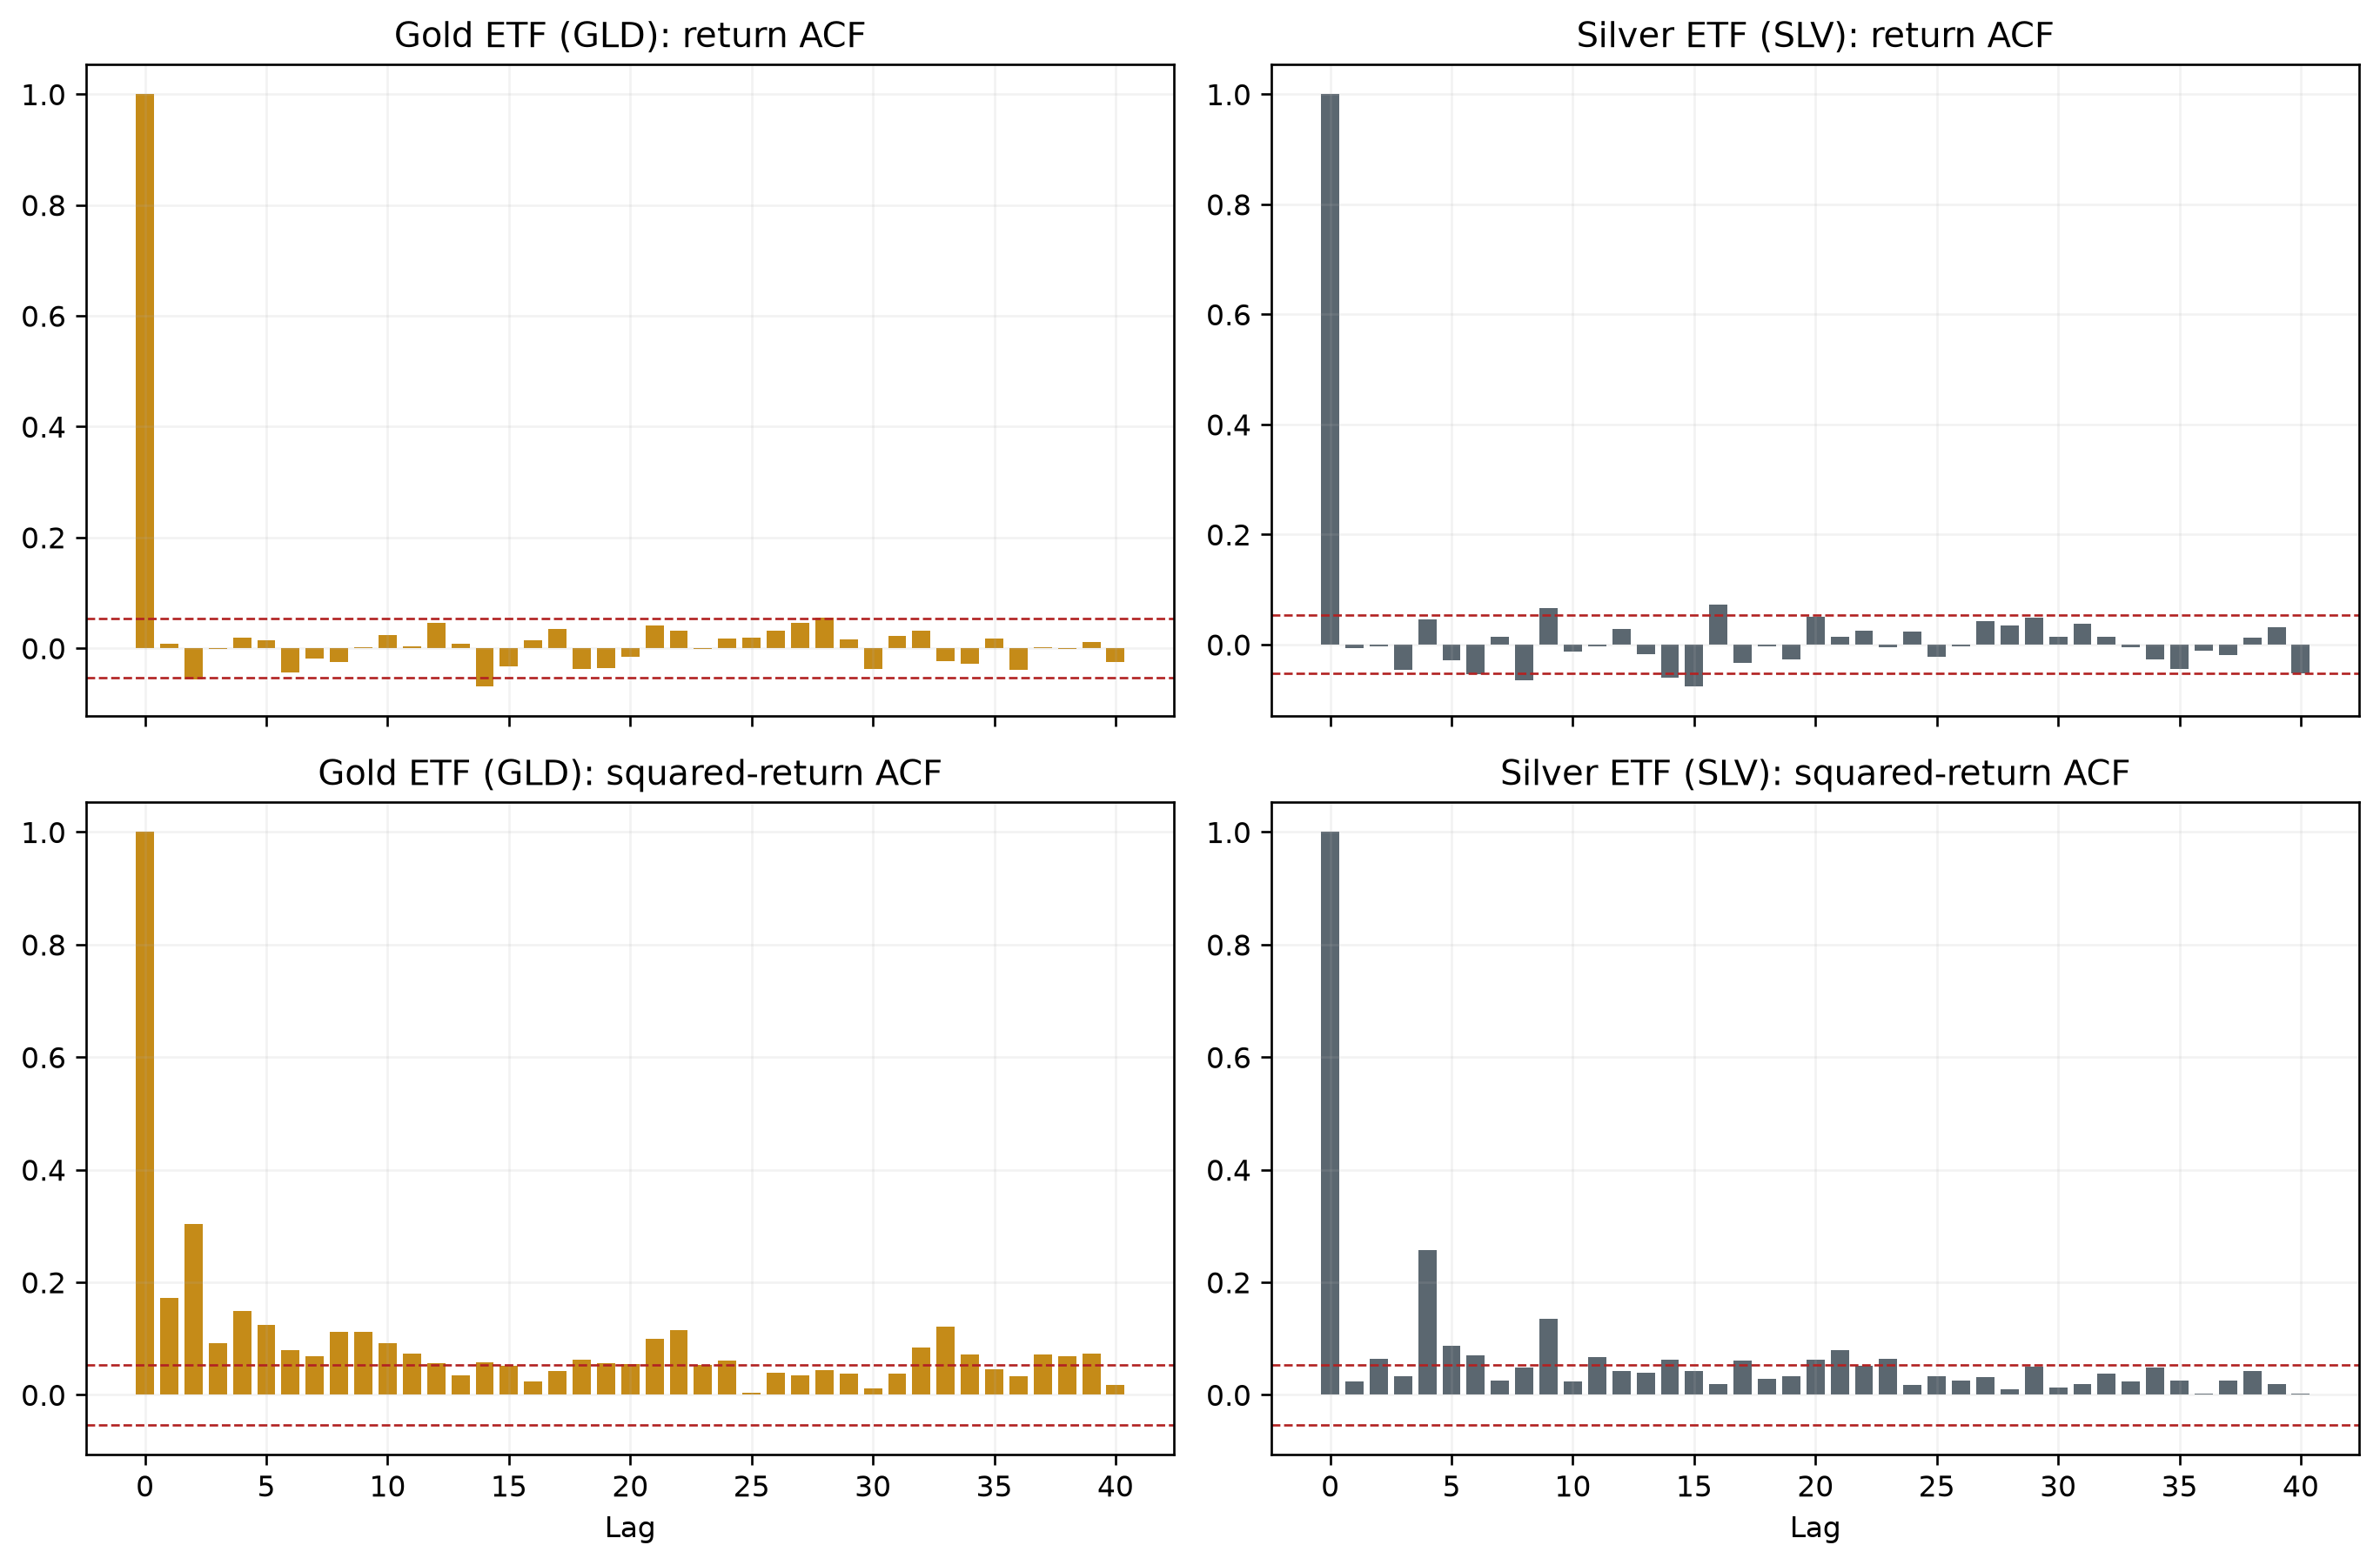
\includegraphics[width=0.95\textwidth]{../img/publication/0bc50334767c3172_acf_grid_gold_silver.png}
\caption{Current LSE autocorrelation diagnostics for GLD/SLV returns and squared returns}
\label{fig:t7-acf-grid}
\end{figure}

\begin{table}[htbp]
\centering
\caption{Short-run volatility-persistence diagnostics}
\label{tab:t7-persistence}
\small
\begin{tabular}{lrrr}
\toprule
Asset & $\hat\phi$ & Robust s.e. & $t$-statistic \\
\midrule
Gold   & 0.115 & 0.020 & 5.60 \\
Silver & 0.156 & 0.024 & 6.40 \\
\bottomrule
\end{tabular}
\begin{minipage}{0.94\textwidth}
\footnotesize\emph{Notes:} OLS estimates from
$|r_t|=c+\phi|r_{t-1}|+\varepsilon_t$, with HC1 standard errors. Values
reproduce the compact persistence table in the Team~7 article.
\end{minipage}
\end{table}

\section{ARCH and GARCH Evidence}

Chapter~\ref{ch:econometrics} defines the ARCH/GARCH family~\cite{Engle1982,Bollerslev1986}; the benchmark here is GARCH$(1,1)$,
\[
 r_t=\mu+\varepsilon_t,\qquad
 \sigma_t^2=\omega+\alpha\varepsilon_{t-1}^2+\beta\sigma_{t-1}^2.
\]
The LSE fit minimizes the Gaussian quasi-negative-log-likelihood
\[
\frac12\sum_t\left[\log h_t+\frac{(r_t-\mu)^2}{h_t}\right],
\qquad h_t=\sigma_t^2,
\]
using percentage-point returns and $h_0=\max(s_r^2,10^{-8})$, with
sample variance $s_r^2$ computed using denominator $N-1$.
L-BFGS-B optimizes $\mu$ and transformed parameters
\[
\omega=e^{\vartheta_1},\quad
\alpha=0.30\ell(\vartheta_2),\quad
\beta=(0.999-\alpha)\ell(\vartheta_3),\qquad
\ell(x)=(1+e^{-x})^{-1}.
\]
Bounds are $\mu\in[-2,2]$, $\vartheta_1\in[-20,4]$ and
$\vartheta_2,\vartheta_3\in[-8,8]$, with a 3,000-iteration cap.
Hence $\alpha<0.30$ and $\alpha+\beta<0.999$ are imposed restrictions.
The table reports the obtained LSE fits, with higher persistence for
SLV. Reported convergence flags certify neither global optimality nor
an unrestricted fit; no robust/Hessian covariance or out-of-sample
assessment is supplied here. The separate ten-day forecasts belong
to the legacy fit.

\begin{table}[htbp]
\centering
\caption{GARCH(1,1) estimates for gold and silver daily returns}
\label{tab:t7-garch-parameters}
\small
\resizebox{0.96\textwidth}{!}{%
\begin{tabular}{lrrrrrr}
\toprule
Asset & $\hat\mu$ & $\hat\omega$ & $\hat\alpha$ & $\hat\beta$
& $\hat\alpha+\hat\beta$ & $\hat\sigma^2_{\infty}$ \\
\midrule
GLD & 0.03494 & 0.05385 & 0.10894 & 0.84798 & 0.95692 & 1.2500 \\
SLV & 0.01495 & 0.04080 & 0.05453 & 0.93900 & 0.99353 & 6.3067 \\
\bottomrule
\end{tabular}}
\begin{minipage}{0.94\textwidth}
\footnotesize\emph{Notes:} Returns and conditional standard deviations
are in percentage points; $\omega$ and variances are in squared
percentage points. With unit-variance standardized innovations and a
stationary finite second moment,
$\sigma_\infty^2=\omega/(1-\alpha-\beta)$.
Values refer to the constrained LSE fit.
\end{minipage}
\end{table}

Figure~\ref{fig:t7-garch-conditional-volatility} shows the regenerated fitted
conditional-volatility paths. Silver fluctuates around a higher baseline and
has larger spikes; for both metals the decay after stress episodes is gradual,
as implied by the near-unit persistence estimates.

\begin{figure}[htbp]
\centering
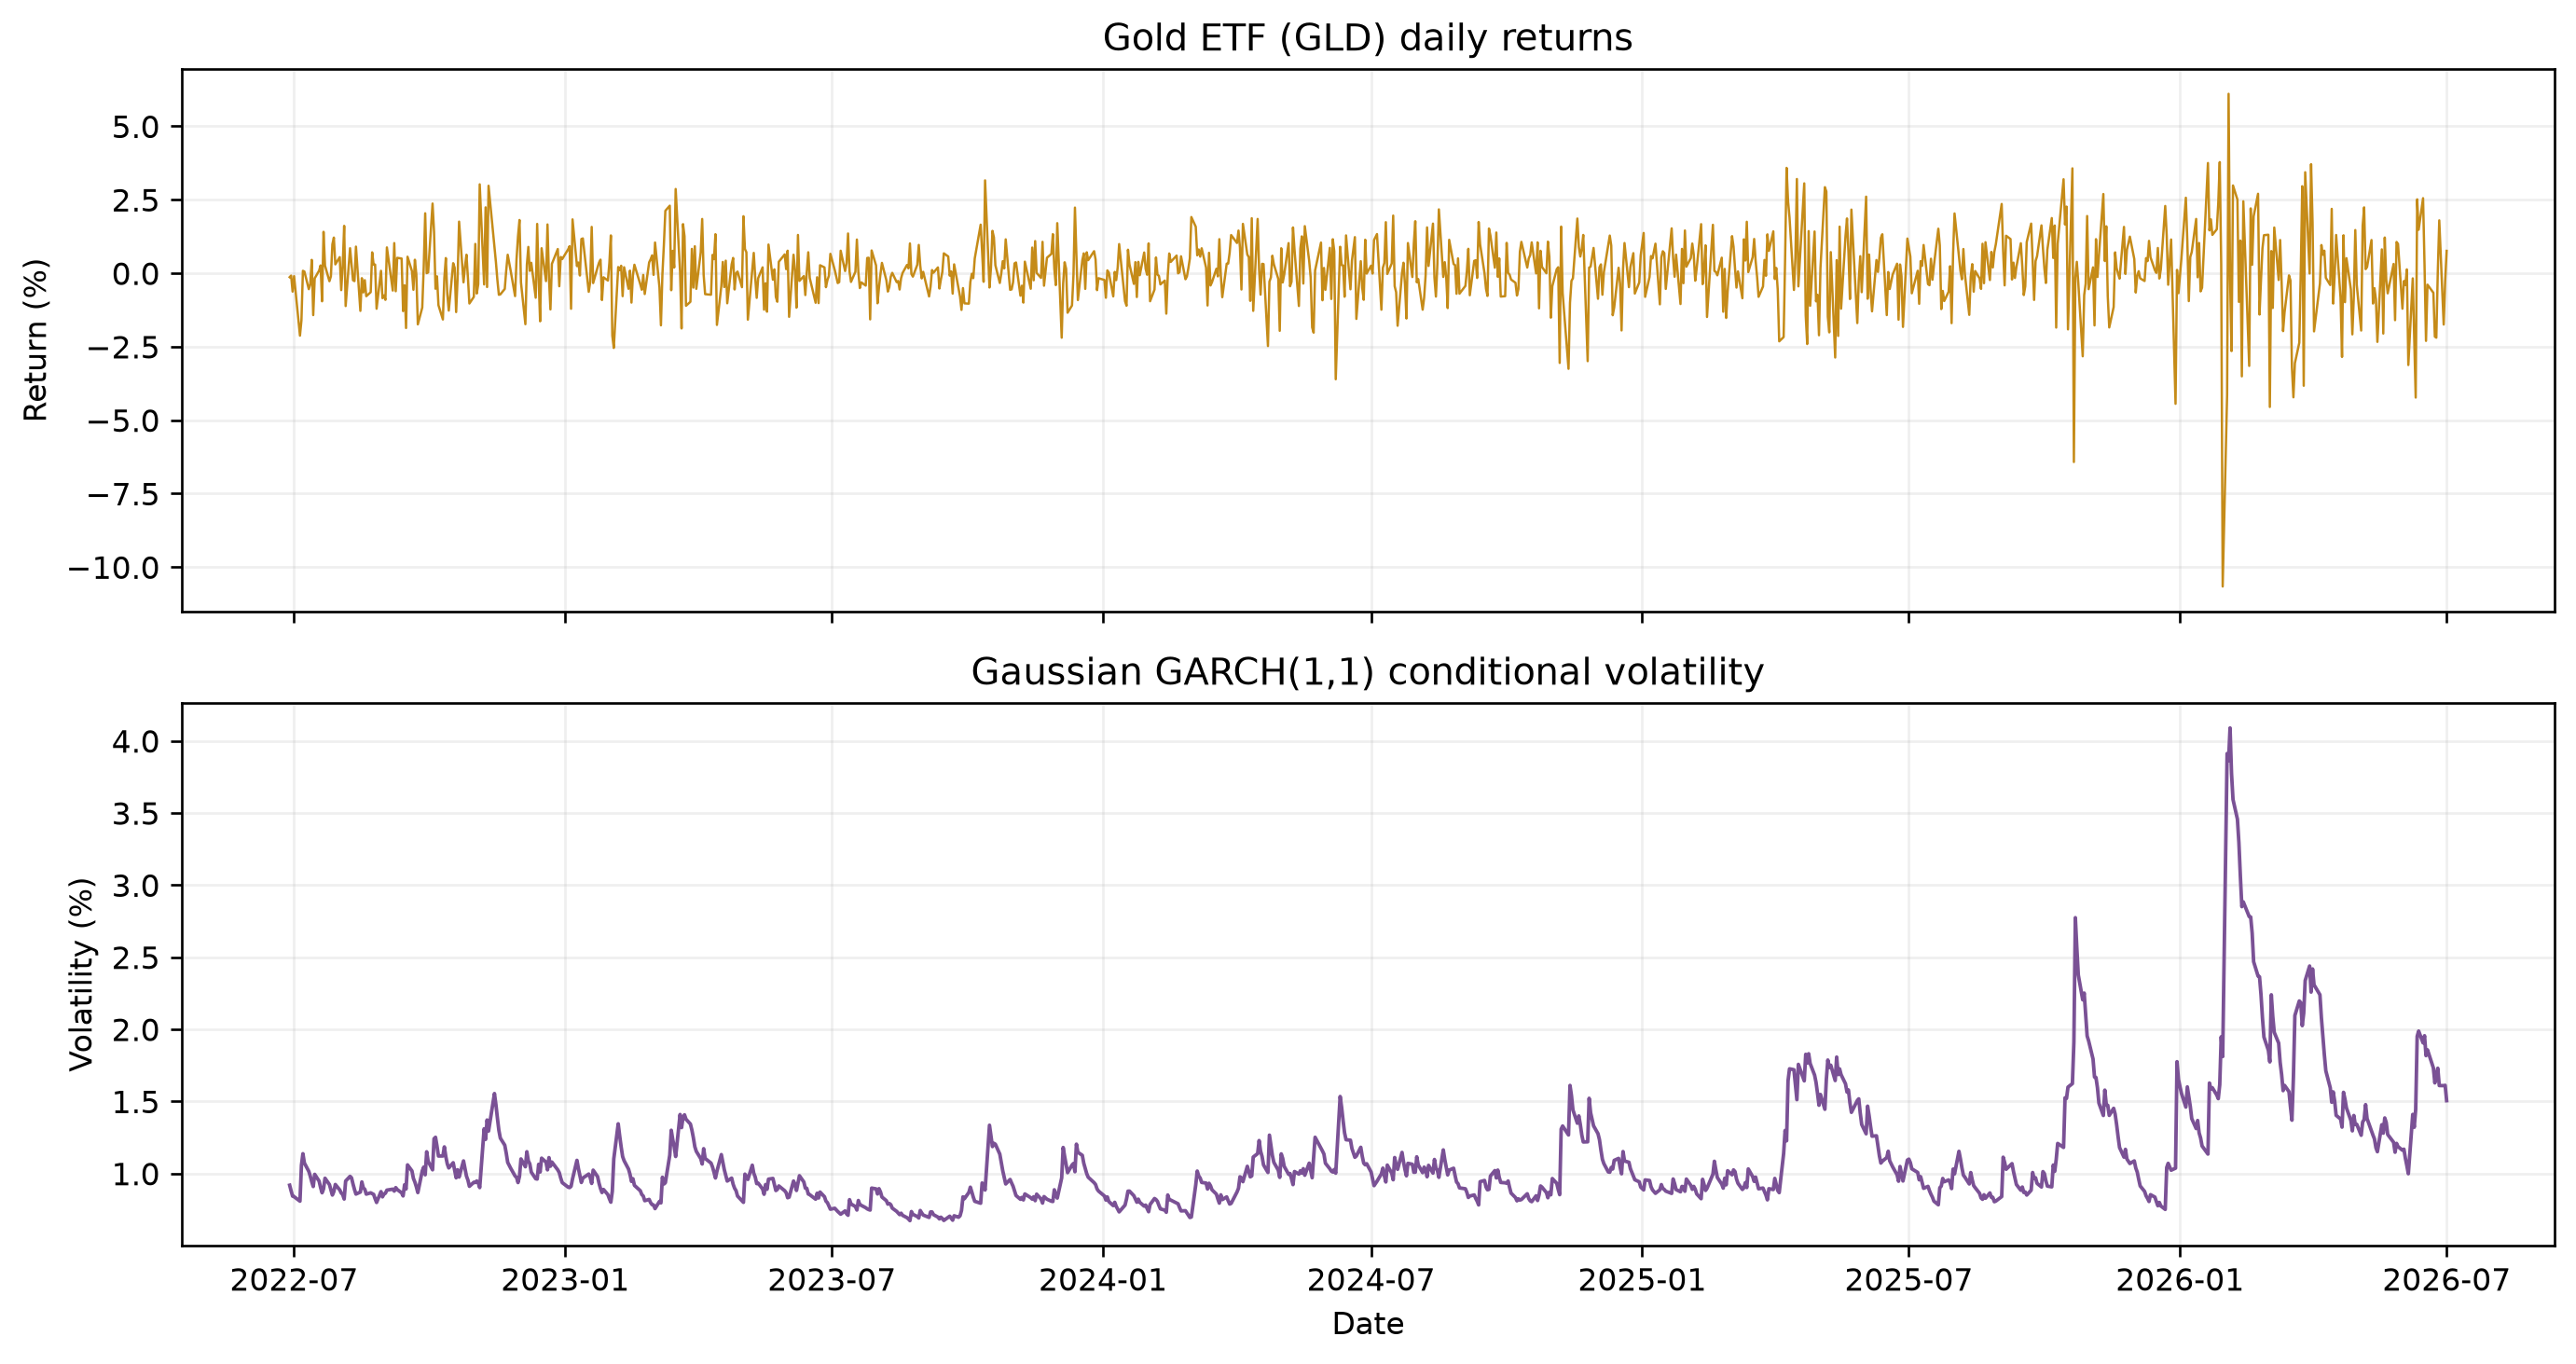
\includegraphics[width=0.90\textwidth]{../img/publication/afc13b2f80014b25_garch_condvol_gold.png}
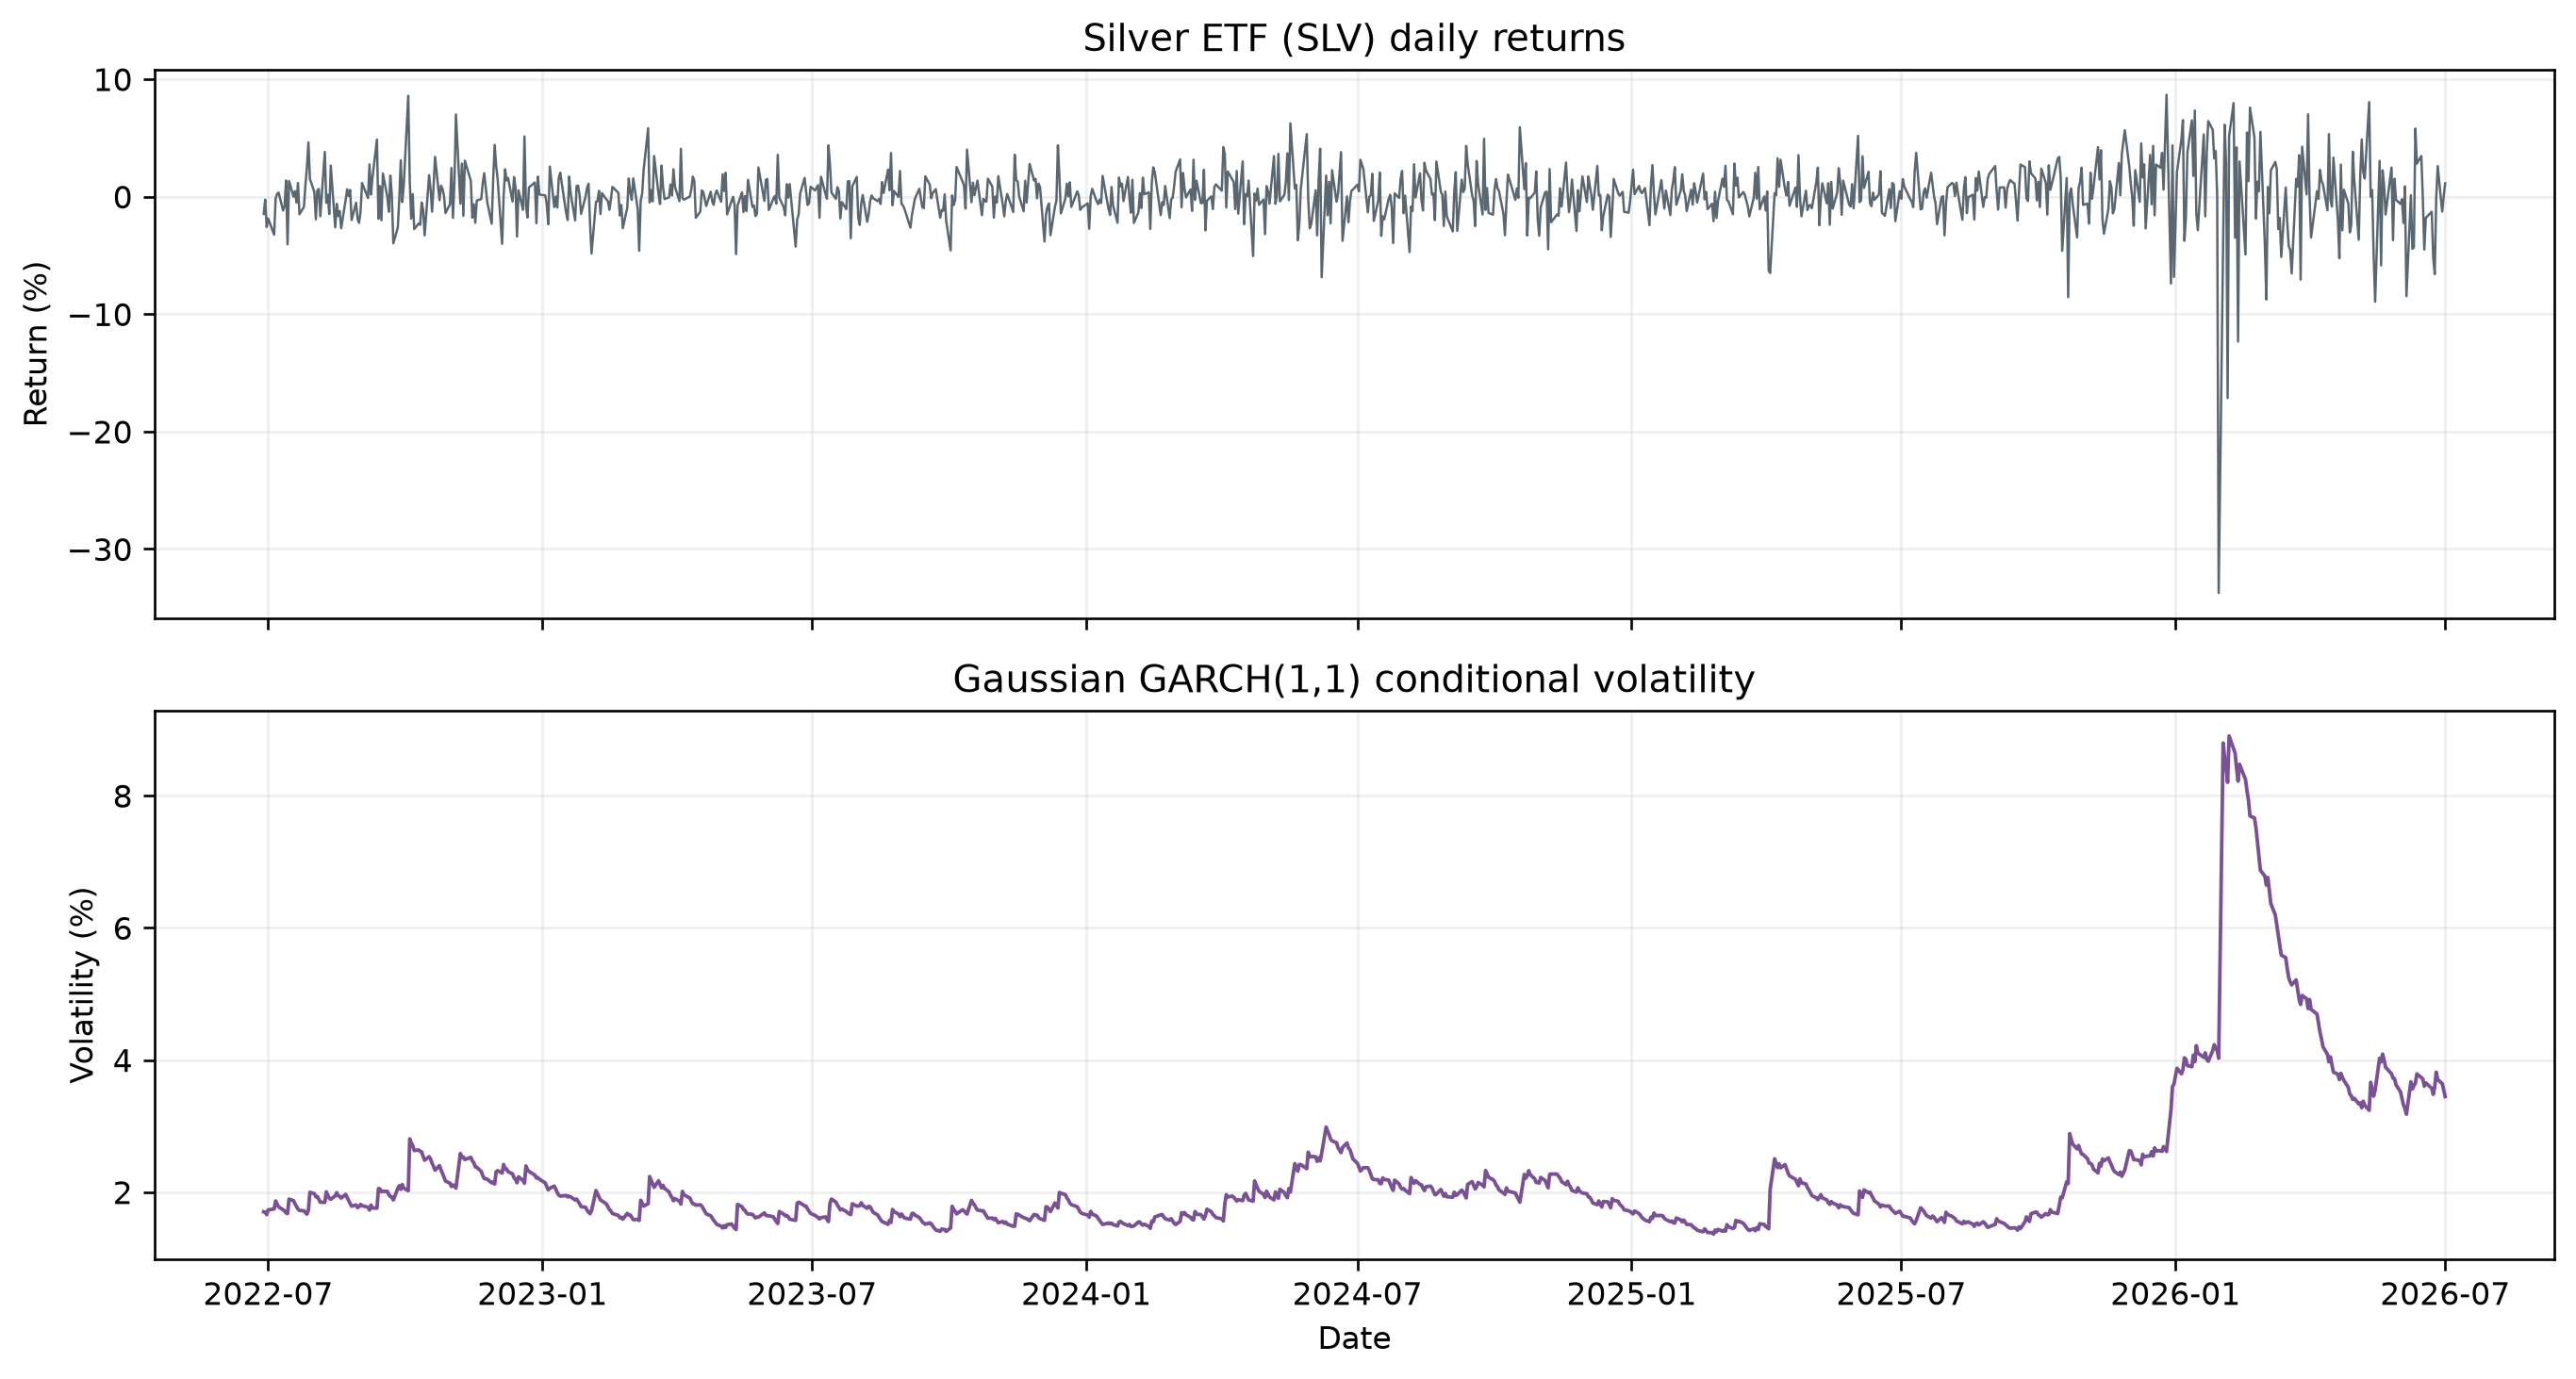
\includegraphics[width=0.90\textwidth]{../img/publication/3b18a0aa9daae0e4_garch_condvol_silver.png}
\caption{Current LSE Gaussian GARCH(1,1) conditional volatility for GLD and SLV}
\label{fig:t7-garch-conditional-volatility}
\end{figure}

For historical comparison, the original Team~7 end-of-sample variance forecasts in
Table~\ref{tab:t7-garch-forecasts} show the same slow mean reversion. In that legacy run, gold
moves from approximately $0.981$ to $1.002$ squared percentage points over ten
days, toward a long-run level of $1.211$; silver moves from $2.686$ to $2.791$,
toward $4.235$.

\begin{table}[htbp]
\centering
\caption{Original Team~7 end-of-sample GARCH conditional-variance forecasts}
\label{tab:t7-garch-forecasts}
\small
\begin{tabular}{crr@{\qquad}crr}
\toprule
$h$ & Gold & Silver & $h$ & Gold & Silver \\
\midrule
1 & 0.981250 & 2.685694 &  6 & 0.993096 & 2.745300 \\
2 & 0.983669 & 2.697803 &  7 & 0.995391 & 2.756943 \\
3 & 0.986064 & 2.709817 &  8 & 0.997662 & 2.768495 \\
4 & 0.988433 & 2.721737 &  9 & 0.999908 & 2.779957 \\
5 & 0.990777 & 2.733565 & 10 & 1.002131 & 2.791329 \\
\bottomrule
\end{tabular}
\begin{minipage}{0.90\textwidth}
\footnotesize\emph{Notes:} Forecast horizon $h$ is measured in trading days;
variances are in squared percentage-return units.
\end{minipage}
\end{table}

These estimates show why GARCH is useful: it converts clustering into a
dynamic conditional-variance forecast. GARCH remains a discrete-time model,
and this is a strength for empirical diagnosis rather than a conceptual flaw.
Its role here is to show that the relevant predictable object is volatility
more than the daily conditional mean.

\section{Long-Memory Cross-Check: GPH and Fractional Differencing}

GARCH captures short-run clustering with a recursive conditional variance. A
separate question is whether a volatility proxy also displays hyperbolically
decaying, long-range dependence of the fractionally integrated type~\cite{GrangerJoyeux1980,Hosking1981}. Team~7 applied the semiparametric
Geweke--Porter--Hudak estimator~\cite{GewekePorterHudak1983} to absolute daily returns. The published
estimates in Table~\ref{tab:t7-gph} are positive and precisely estimated. The
current LSE figure rebuild no longer clips the estimate at an implementation
boundary. Its unclipped estimates are $\hat d=\GphGoldAbs$ for GLD and
$\hat d=\GphSilverAbs$ for SLV; it does not reuse the published point
estimates.

\begin{table}[htbp]
\centering
\caption{Original Team~7 GPH estimates of the fractional differencing parameter for absolute returns}
\label{tab:t7-gph}
\small
\begin{tabular}{lrrr}
\toprule
Asset & $\hat d$ & s.e.($\hat d$) & $t$-statistic \\
\midrule
Gold   & 0.576 & 0.090 & 6.39 \\
Silver & 0.552 & 0.080 & 6.91 \\
\bottomrule
\end{tabular}
\end{table}

The absolute-return ACF in Figure~\ref{fig:t7-absolute-return-acf}
and filtered series in Figure~\ref{fig:t7-fractional-differencing}
are descriptive LSE diagnostics; a visual change after filtering alone
does not establish reduced low-frequency persistence. The finite filter,
a truncation of $(1-B)^d=\sum_{k\ge0}w_kB^k$ with backshift operator $B$,
$w_0=1$ and $w_k=-w_{k-1}(d-k+1)/k$, assigns weight $w_0$ to the current observation and subsequent weights
to past observations. With $L$ retained weights, its first $L-1$ values
are undefined (599 if $L=600$), so the filtered sample differs from
the full sample used for the raw GPH slope.

\begin{figure}[htbp]
\centering
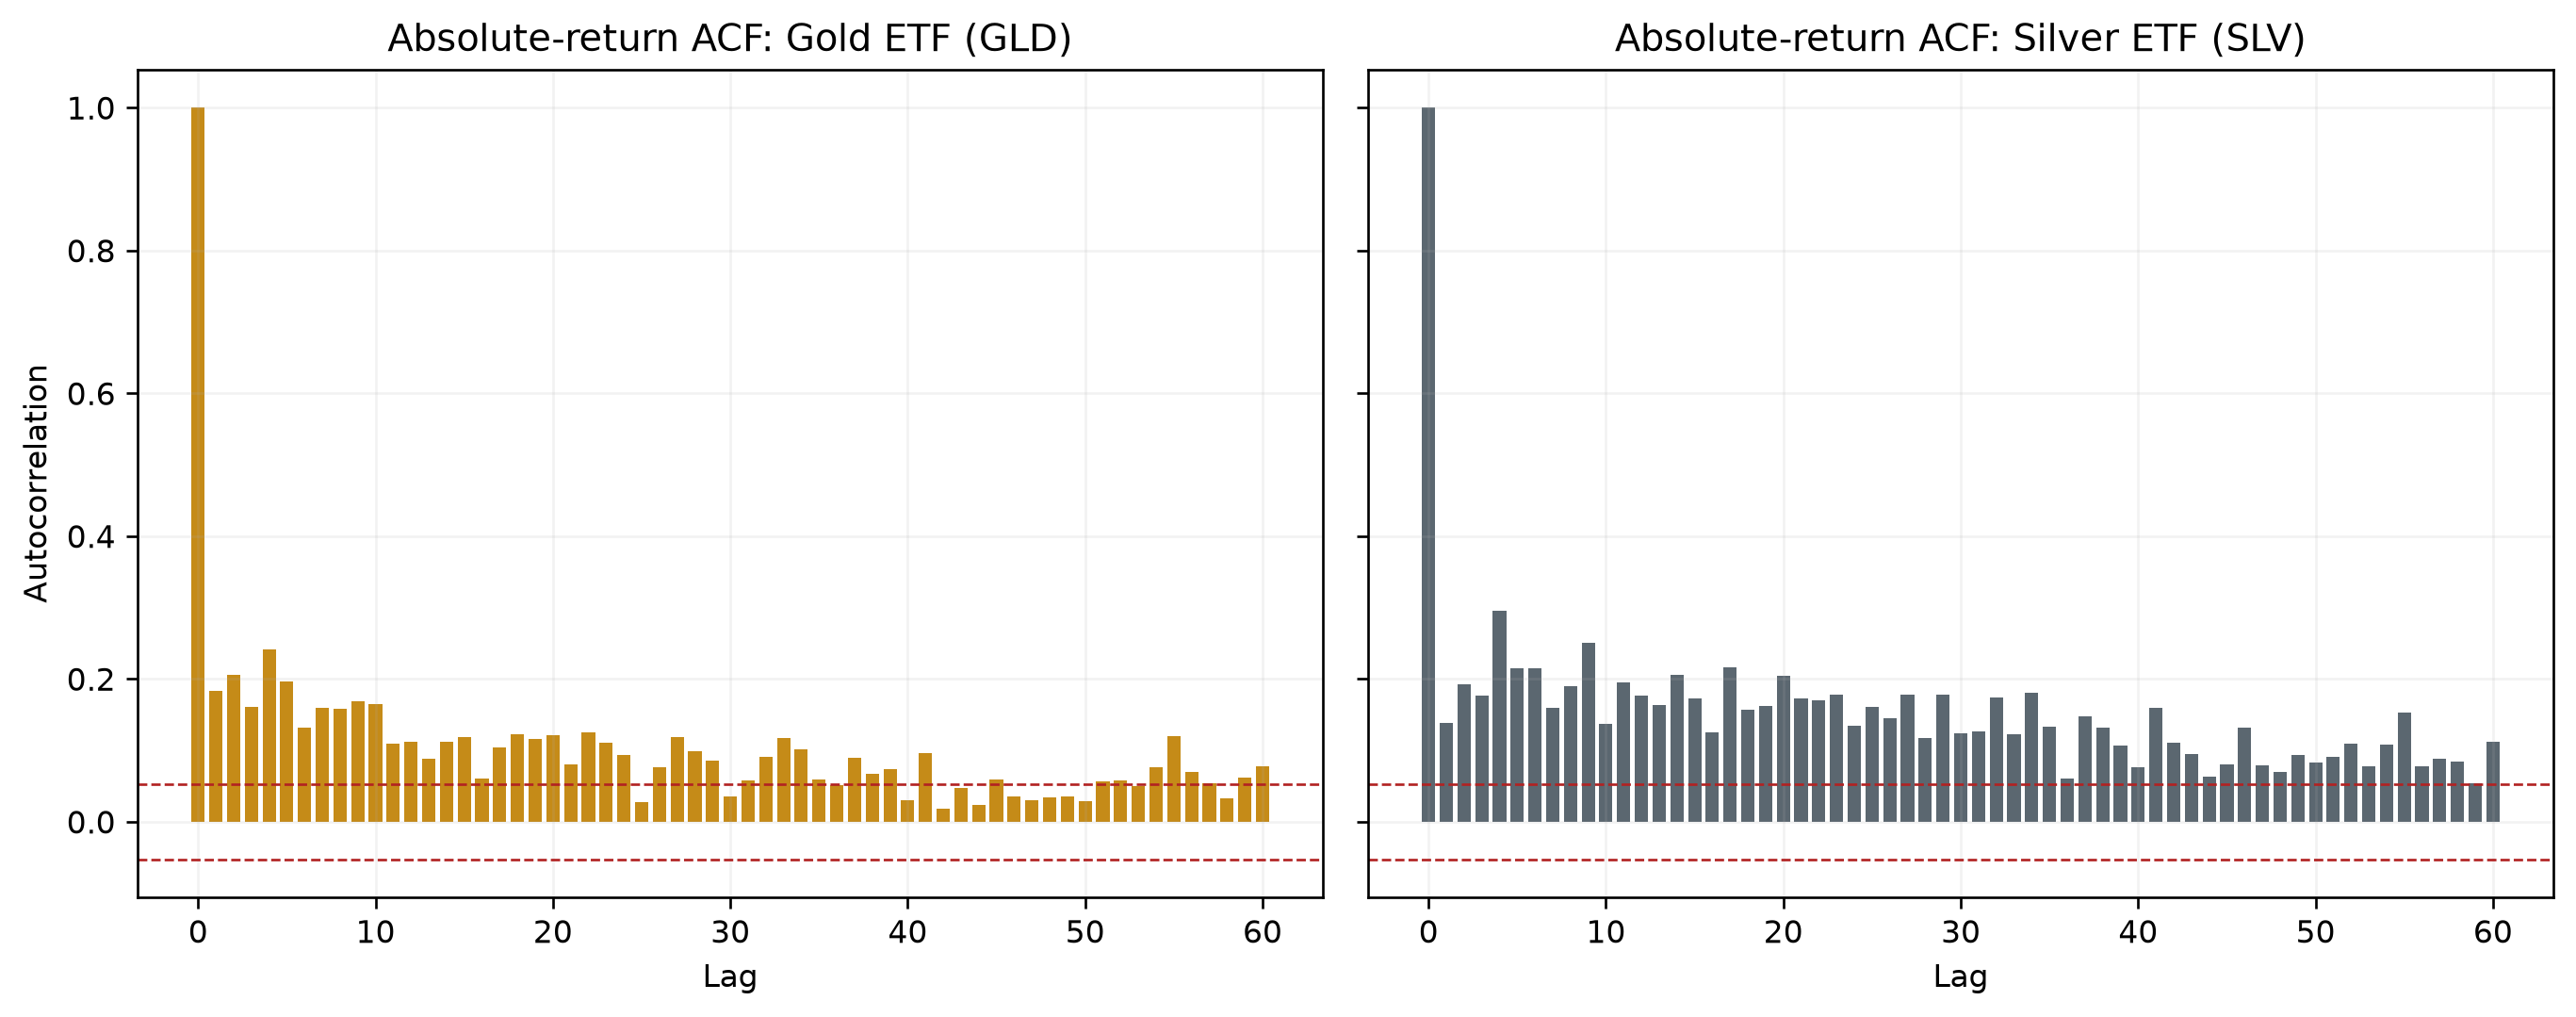
\includegraphics[width=0.88\textwidth]{../img/publication/947d32538e7a36b6_acf_abs_returns_gold_silver.png}
\caption{Current LSE autocorrelation functions of GLD and SLV absolute returns}
\label{fig:t7-absolute-return-acf}
\end{figure}

\begin{figure}[htbp]
\centering
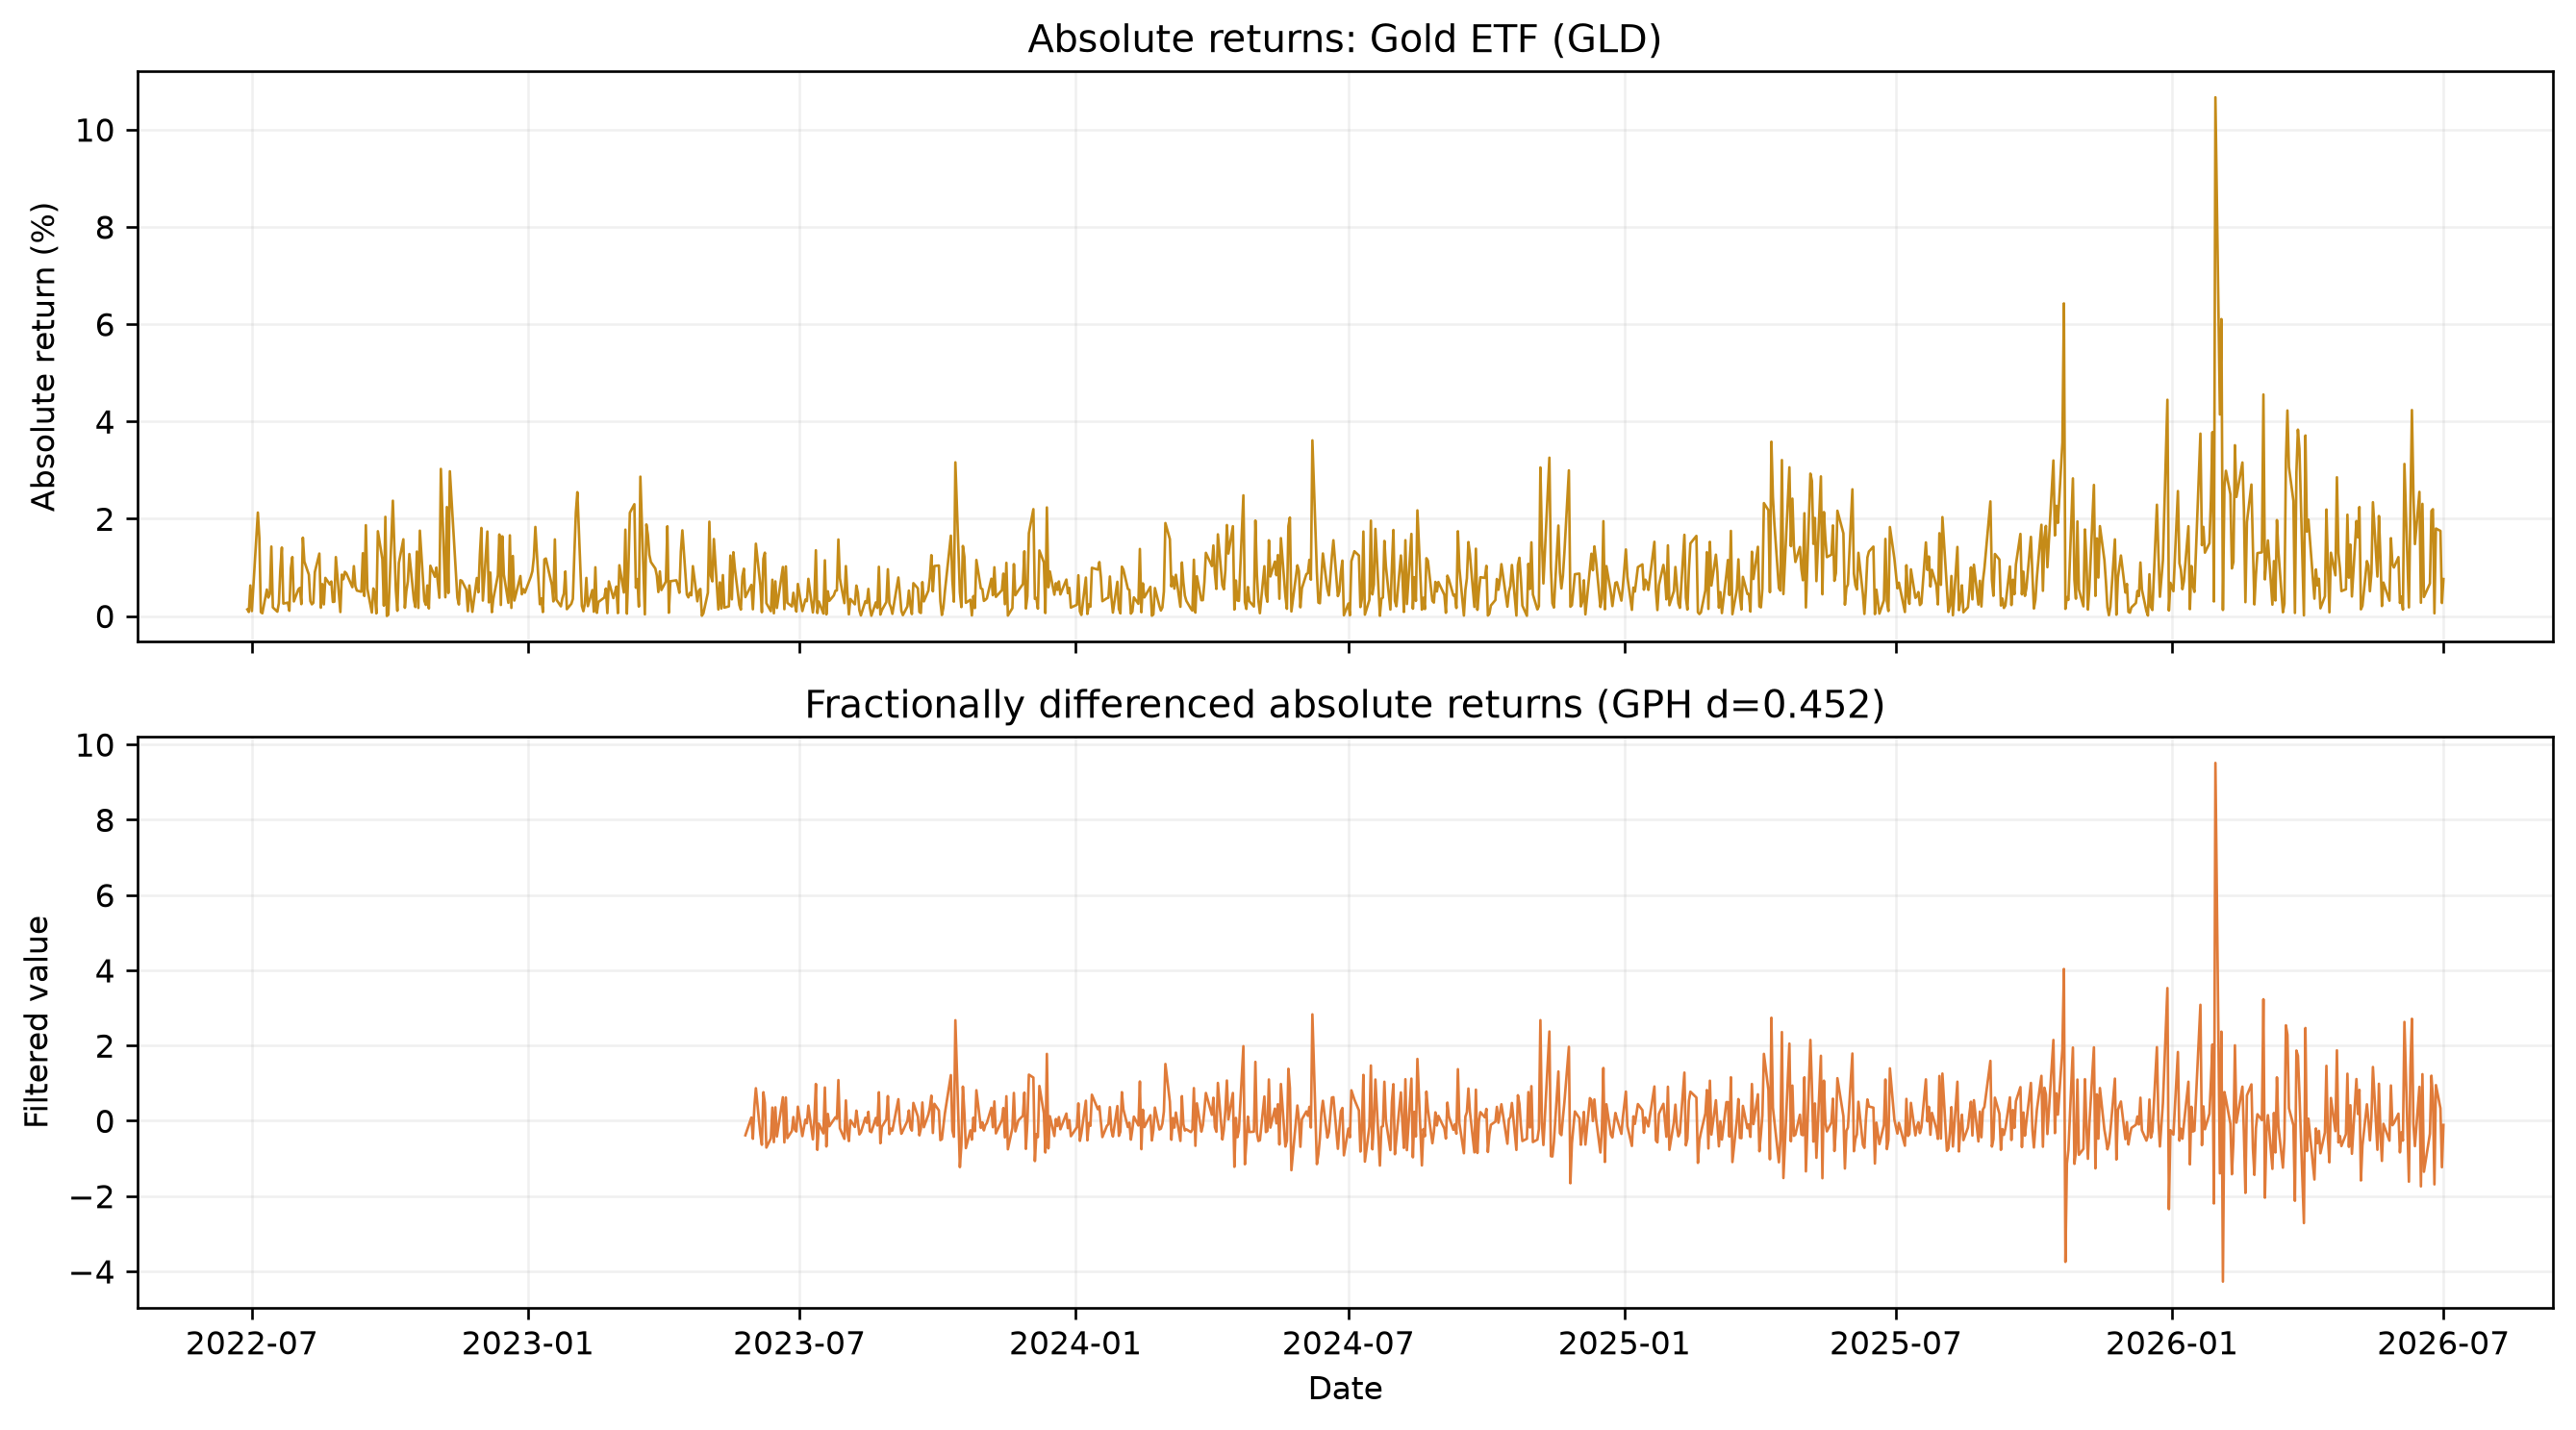
\includegraphics[width=0.86\textwidth]{../img/publication/1ed7701f31854135_arfima_fd_gold.png}
\includegraphics[width=0.86\textwidth]{\FigArfimaFdSilver}
\caption{Current LSE absolute returns and fractional filtering; the plotted unclipped GPH estimates are \GphGoldAbs{} for GLD and \GphSilverAbs{} for SLV}
\label{fig:t7-fractional-differencing}
\end{figure}

The result requires a stronger qualification than the original standalone
article supplied. In the elementary ARFIMA case, covariance stationarity
requires $d<0.5$; both published point estimates exceed that boundary.
The current GLD estimate lies below it, whereas the unclipped SLV estimate
lies in the non-stationary range $d>0.5$, in line with the published silver
estimate. The evidence is therefore compatible with very strong or
boundary-sensitive persistence, but it does not establish a stable
covariance-stationary ARFIMA law, least of all for silver.
Bandwidth sensitivity, alternative long-memory estimators and structural-break
controls remain necessary before assigning a stable economic interpretation.

\clearpage
\section{Limitations and Downstream Resolution}

\paragraph{Limitations of this empirical layer.}
The evidence is conditional on daily frequency and ETF proxies for spot
metals. The chapter deliberately juxtaposes the published Yahoo-based tables with current
LSE figures; their estimates are not pooled. Calendar synchronization, the
SPY and DXY-formula proxies, and the use of a yield change alongside asset
returns affect interpretation.
Static and rolling correlations and HC1 regressions are descriptive; they do
not identify monetary, inflationary or geopolitical shocks. Normal-innovation
GARCH does not represent leverage asymmetry, heavy-tailed innovations,
structural breaks or jump arrivals. The GPH result is boundary-sensitive. The
published AR(1) robust standard errors differ from the Newey--West HAC values
of the corrected companion code (Table~\ref{tab:t7-ar1-level-return}); the
small excess-kurtosis difference noted under Table~\ref{tab:t7-return-moments}
remains unexplained. No estimates are recomputed here.

\paragraph{Residual research agenda.}
Work that remains genuinely open includes a same-date, multi-provider rebuild
of the historical panel; Student-$t$, asymmetric and regime-switching
volatility benchmarks; rolling or expanding-window re-estimation; formal
causal identification of macroeconomic shocks; and robust long-memory tests
under breaks. The most important interface question is the mapping between
historical $\mathbb P$ dynamics and option-implied $\mathbb Q$ parameters.
An augmented filtration that converts textual macroeconomic and geopolitical
information into measurable state variables is also a credible machine-
learning extension, but it is outside the evidence completed in this thesis.
Additional regressors, quantile methods and formal regime identification
likewise remain extensions rather than completed results.

The decision point is therefore precise. ARIMA remains valid for integrated
levels and GARCH remains useful for discrete-time conditional variance, but
low-dimensional historical mean models cannot jointly represent the option
smile, continuous stochastic variance and discontinuous repricing required by
the valuation. Chapter~\ref{ch:sv-jumps} introduces that model layer without treating an
option-implied distribution as an automatic physical-measure forecast.
